% Created 2016-03-27 Sun 11:52
\documentclass[9pt]{beamer}
\usepackage[utf8]{inputenc}
\usepackage[T1]{fontenc}
\usepackage{fixltx2e}
\usepackage{graphicx}
\usepackage{longtable}
\usepackage{float}
\usepackage{wrapfig}
\usepackage{soul}
\usepackage{textcomp}
\usepackage{marvosym}
\usepackage{wasysym}
\usepackage{latexsym}
\usepackage{amssymb}
\usepackage{hyperref}
\tolerance=1000
\mode<beamer>{\usetheme{Warsaw}}
\mode<beamer>{\setbeamertemplate{blocks}[rounded][shadow=false]}
\mode<beamer>{\addtobeamertemplate{block begin}{\pgfsetfillopacity{0.8}}{\pgfsetfillopacity{1}}}
\mode<beamer>{\setbeamercolor{structure}{fg=orange}}
\mode<beamer>{\setbeamercovered{transparent}}
\AtBeginSection[]{\begin{frame}<beamer>\frametitle{Topic}\tableofcontents[currentsection]\end{frame}}
\usepackage{subcaption}
\usepackage{multimedia}
\usepackage{tikz}
\usepackage{subfigure,subfigmat}
\usepackage{threeparttable}
\usetikzlibrary{shapes,arrows,shadows}
\usepackage{bm, amssymb, amsmath, array, pdfpages}
\newcommand{\bv}[1]{\mathbf{#1}}
\newcommand{\diff}[2]{\frac{\partial #1}{\partial #2}}
\newcommand{\beq}[0]{\begin{equation}}
\newcommand{\eeq}[0]{\end{equation}}
\newcommand{\beqa}[0]{\begin{eqnarray}}
\newcommand{\eeqa}[0]{\end{eqnarray}}
\newcommand{\beqq}[0]{\begin{equation*}}
\newcommand{\eeqq}[0]{\end{equation*}}
\newcommand{\bs}[1]{\boldsymbol{#1}}
\newcommand{\ip}[2]{\langle #1, #2\rangle}
\providecommand{\alert}[1]{\textbf{#1}}

\title{Modeling and Uncertainty Quantification for Airfoil Icing}
\author{Anthony DeGennaro \newline Clarence W. Rowley III \newline Luigi Martinelli \newline Princeton University}
\date{Group Presentation \\ Princeton, NJ \\ March 2016}
\hypersetup{
  pdfkeywords={},
  pdfsubject={},
  pdfcreator={Emacs Org-mode version 7.9.3f}}

\begin{document}

\maketitle

\begin{frame}
\frametitle{Outline}
\setcounter{tocdepth}{3}
\tableofcontents
\end{frame}



% Define my settings

\graphicspath{{Figures/}}
% Add Princeton shield logo
\addtobeamertemplate{frametitle}{}{%
\begin{tikzpicture}[remember picture,overlay]
\node[anchor=north east,yshift=2pt] at (current page.north east) {
\includegraphics[height=0.7cm]{Shield}};
\end{tikzpicture}}
%


\institute{Princeton University}


\section{Motivation/Background}
\label{sec-1}
\begin{frame}
\frametitle{Introduction}
\label{sec-1-1}

\textbf{Motivation}
\begin{itemize}
\item Wing icing deteriorates airfoil aerodynamics
\begin{itemize}
\item Leading edge flow separation bubble
\item Lower lift, higher drag
\item Unpredictable stall
\end{itemize}
\end{itemize}

\vspace*{-0.0cm}\begin{figure}
    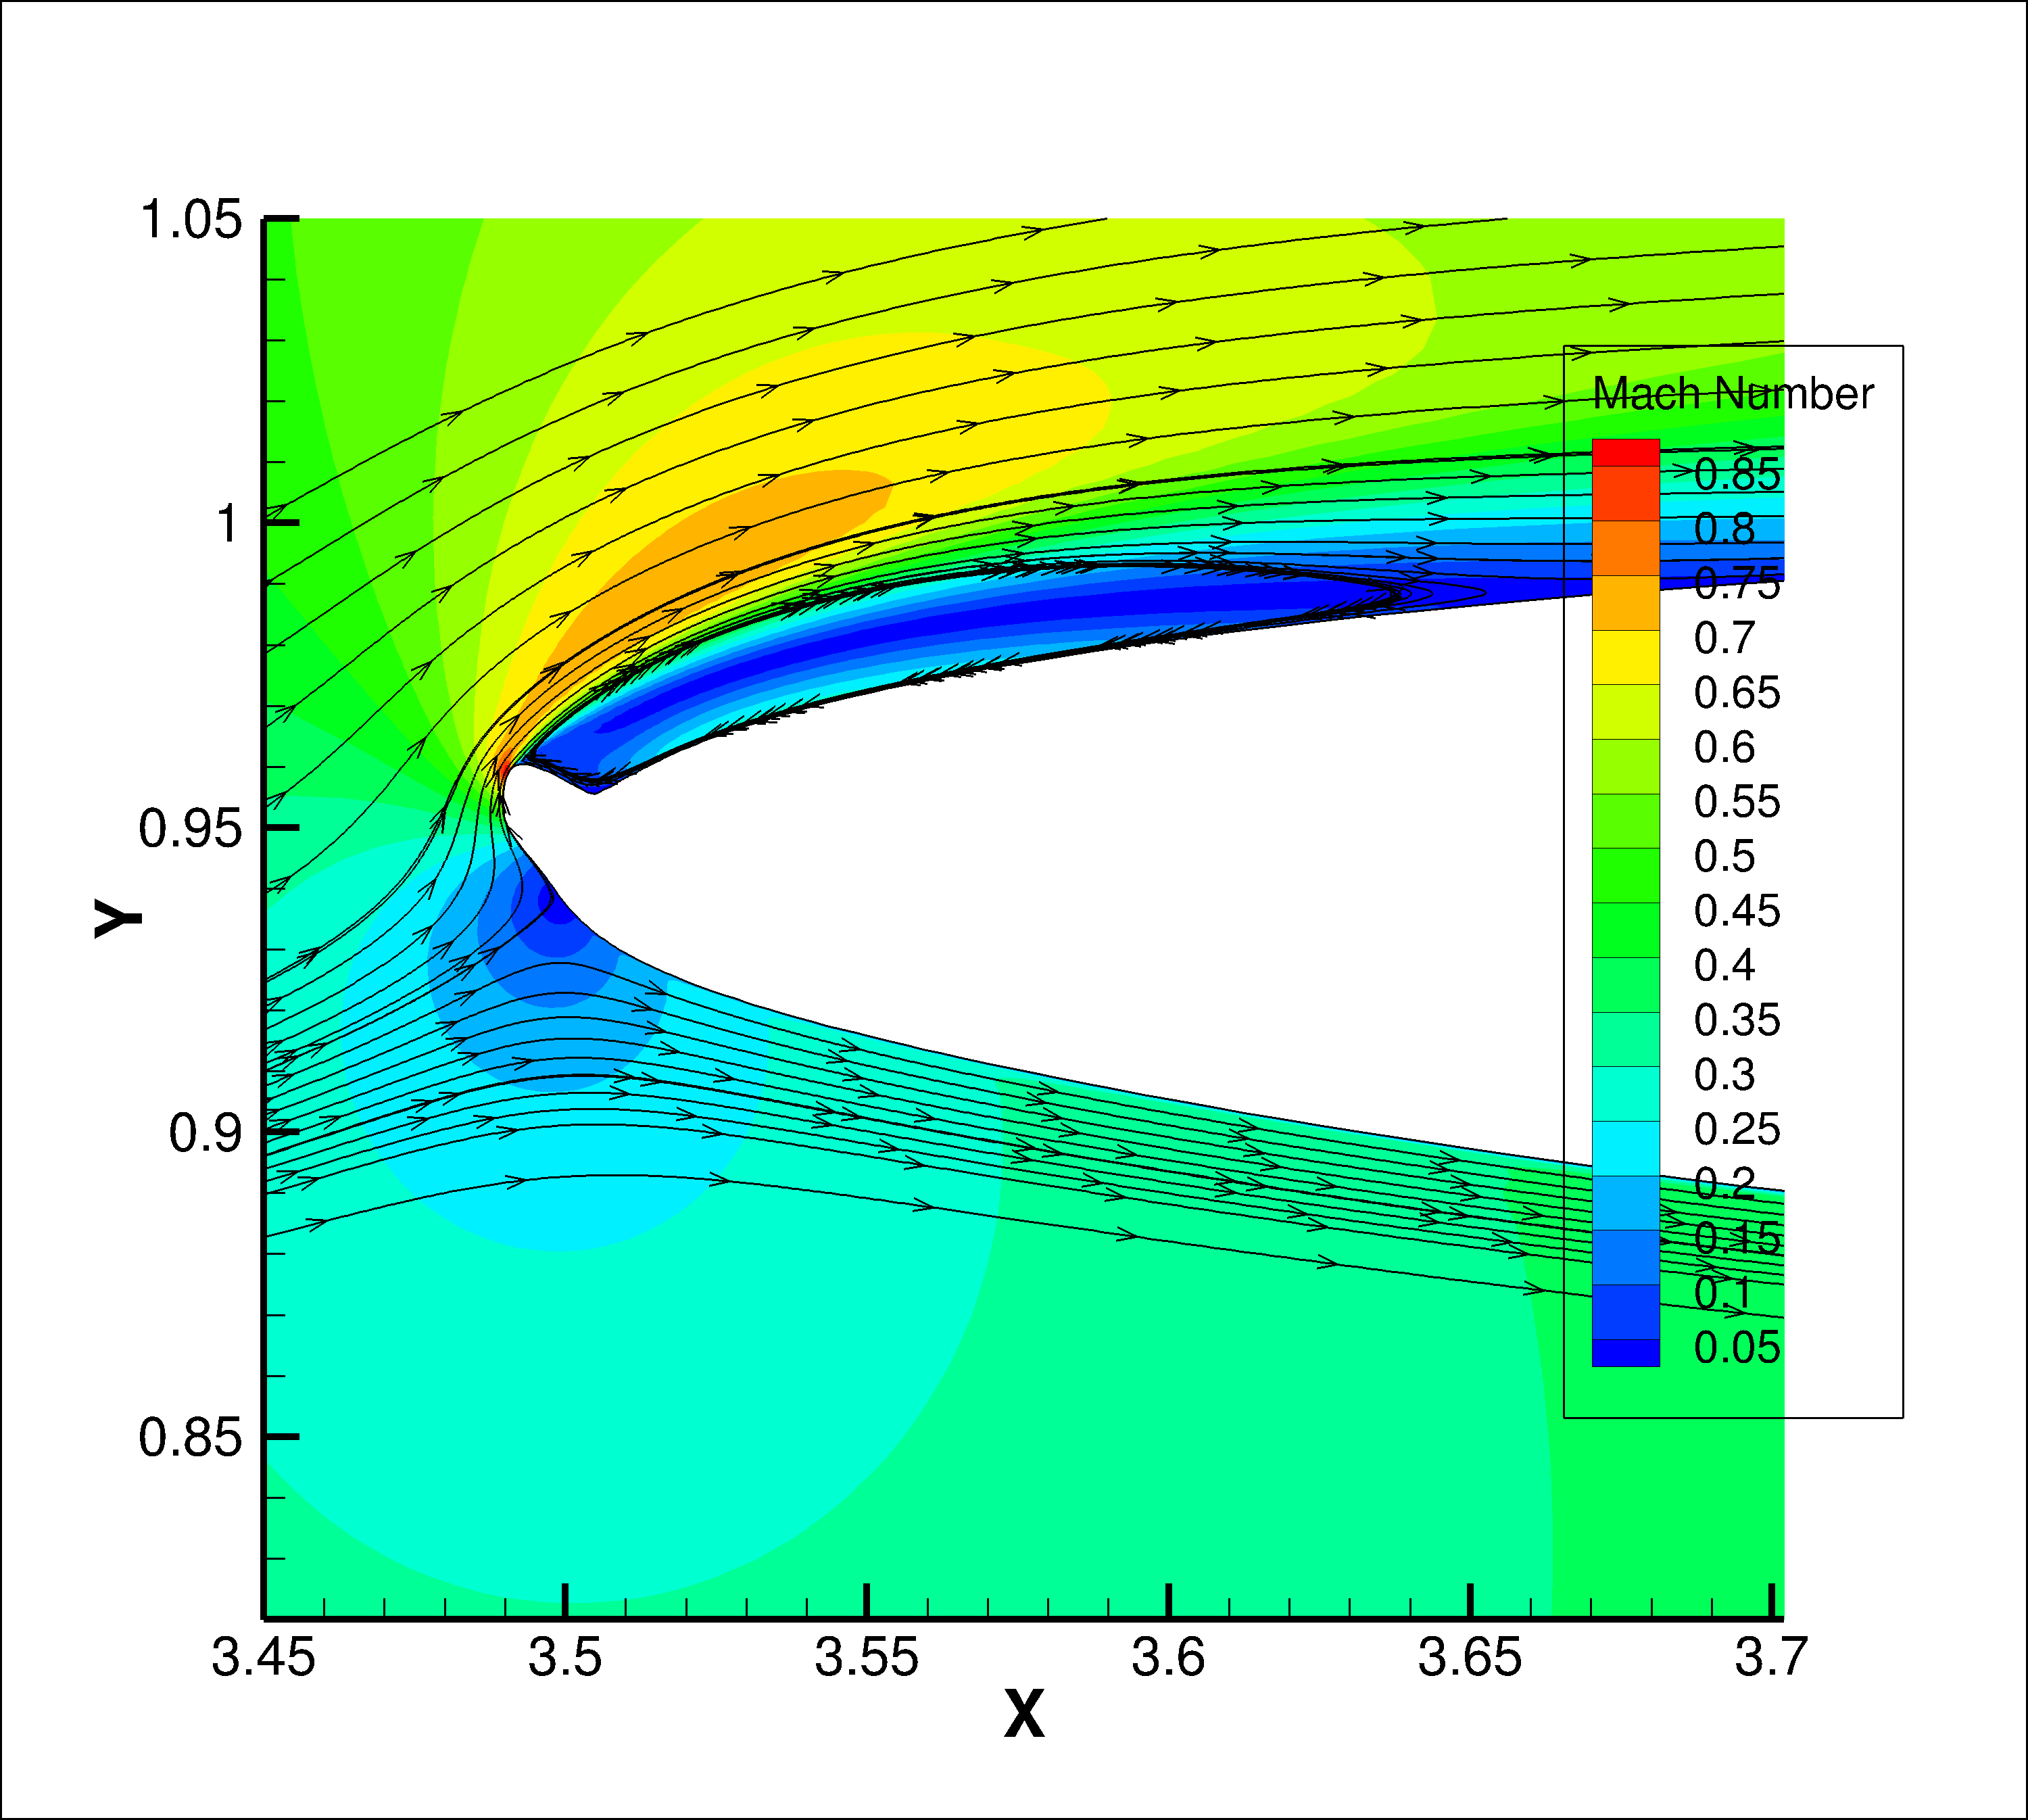
\includegraphics[width=0.4\textwidth]{BadHorn.png}
    \caption{Leading edge horn separation}
\end{figure}
\end{frame}
\begin{frame}
\frametitle{Introduction}
\label{sec-1-2}

\textbf{Motivation}
\begin{itemize}
\item Significant ice shape variation, sensitivity to physical
  parameters\footnote{Addy, H.E. \emph{Ice Accretions and Icing Effects for Modern Airfoils}. NASA TR 2000-210031.
 }
\begin{itemize}
\item Complex physics (aero-thermodynamics, macro/micro scale physics)
\item Uncertainty in physical parameters
\end{itemize}
\end{itemize}

\vspace*{-0.0cm}\begin{figure}
      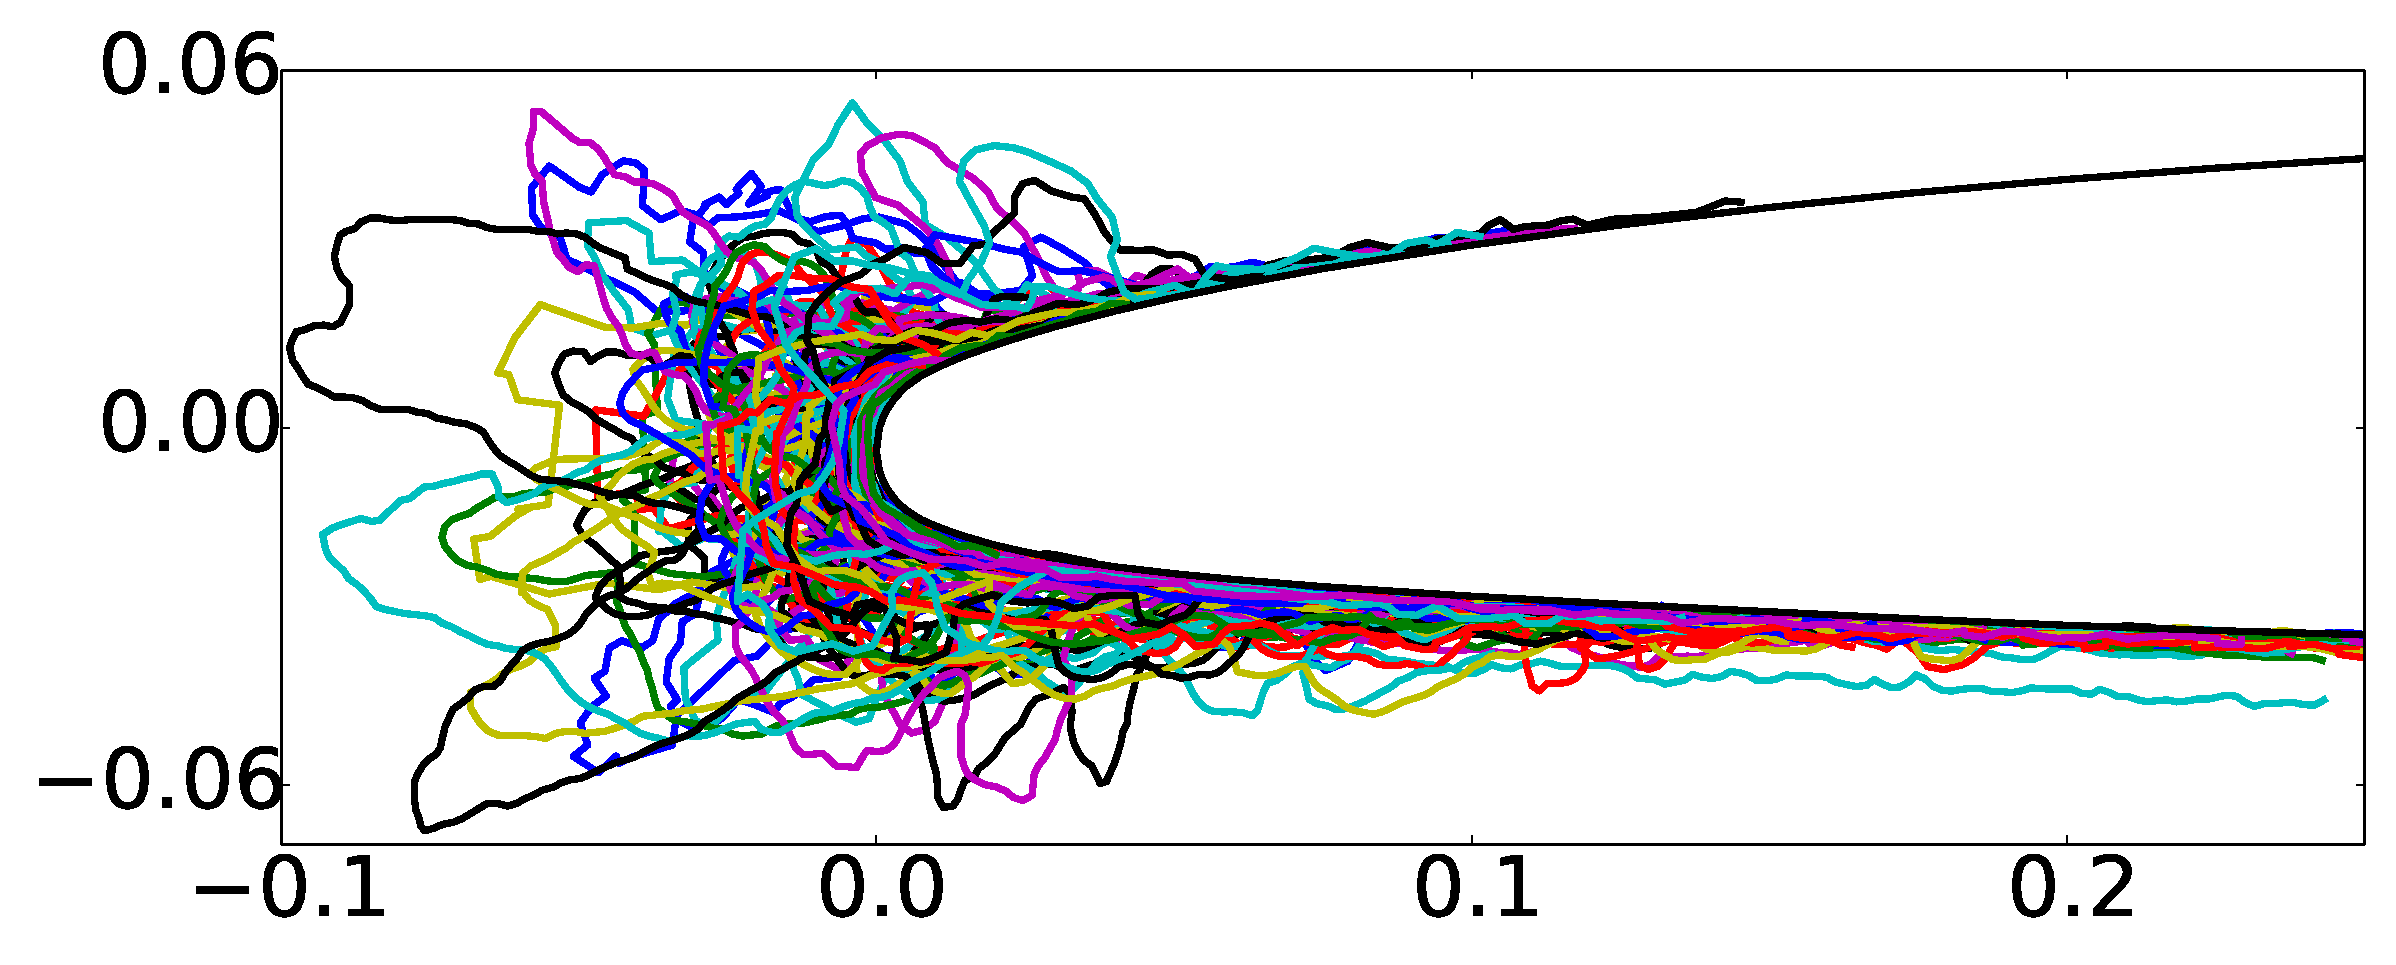
\includegraphics[width=0.75\textwidth]{GlobalDataSet}
      \caption{Wind tunnel experimental ice shapes}
\end{figure}
\end{frame}
\begin{frame}
\frametitle{Introduction}
\label{sec-1-3}

\textbf{Motivation}
\begin{itemize}
\item There appear to be different types of ice accretion\footnote{Beaugendre et. al. \emph{Development of a Second Generation In-Flight Simulation Code}. J. Fluids Engineering, 2006.
 }
\begin{itemize}
\item ``Horns'', ``ridges'', ``lobster tails'' refer to shape
\item ``Glaze'', ``rime'' refer to icing thermodynamics
\end{itemize}
\end{itemize}

\vspace*{-0.0cm}\begin{figure}
      \subfigure[Rime Ice]{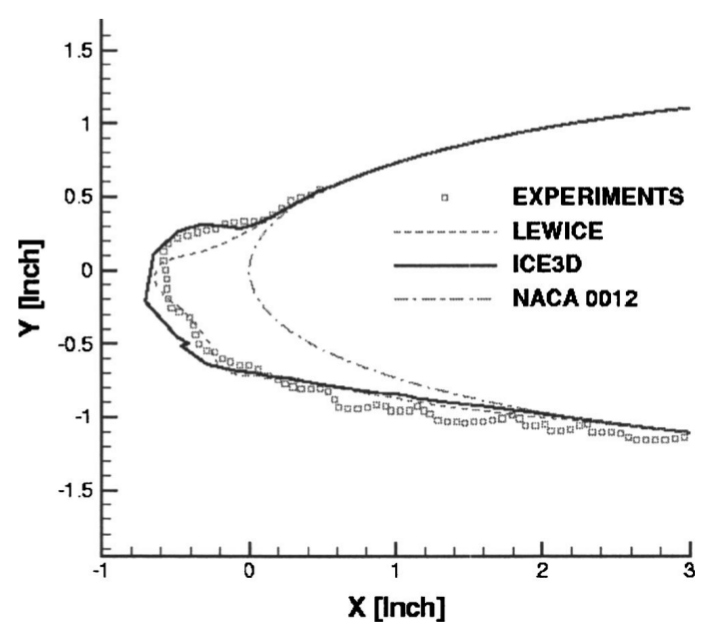
\includegraphics[width=0.4\textwidth]{Habashi2006Rime.png}}
      \subfigure[Horn Ice]{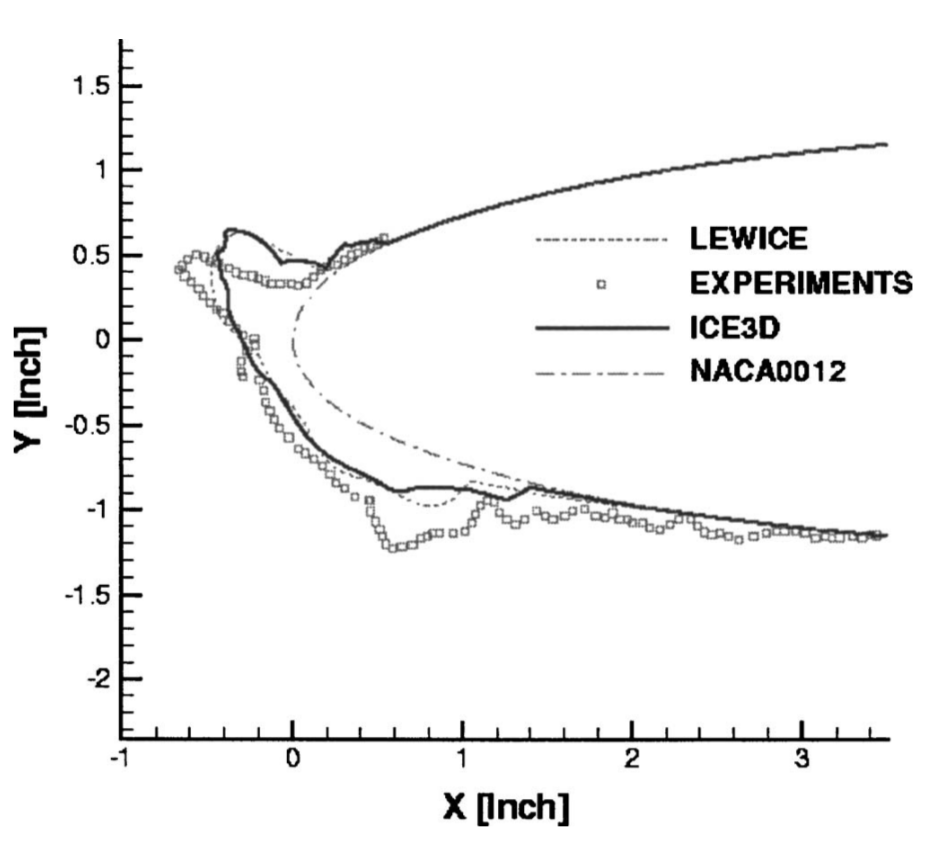
\includegraphics[width=0.4\textwidth]{Habashi2006Horn.png}}
 
\end{figure}
\end{frame}
\begin{frame}
\frametitle{Introduction}
\label{sec-1-4}

\textbf{Research Goals}
\begin{itemize}
\item Apply clustering techniques to segregate database of ice shape data
  into similar groups
\item Build low-dimensional models of resulting clusters
\item Perform parametric uncertainty quantification to understand
  aerodynamic performance variation
\end{itemize}
\end{frame}
\section{Clustering Techniques}
\label{sec-2}
\begin{frame}
\frametitle{Spectral Graph Partitioning}
\label{sec-2-1}

\textbf{Goal:} given an undirected graph $\mathcal{G}$, consisting of a
  collection of vertices $\mathcal{V}$ and corresponding edges
  $\mathcal{E}$, find (or approximate) the ``best'' partition of that
  graph into two connected subgraphs
\vspace*{-0.5cm}\begin{figure}
    \includegraphics[width=0.5\textwidth]{GraphPartition.png}
    \caption{Graph partition illustration}
\end{figure}
\end{frame}
\begin{frame}
\frametitle{Spectral Graph Partitioning}
\label{sec-2-2}

Different formulations possible\footnote{Shi \& Malik. \emph{Normalized Cuts and Image Segmentation}, 2000.
 }
\begin{itemize}
\item \emph{Average cut:} $P(A,B) = \text{min}_{A \subset \mathcal{V}} \left \lbrace \frac{\text{cut}(A,B)}{| A |} + \frac{\text{cut}(A,B)}{| B |} \right \rbrace$
\item \emph{Normalized cut:} $P(A,B) = \text{min}_{A \subset \mathcal{V}} \left \lbrace \frac{\text{cut}(A,B)}{\text{assoc}(A,V)} + \frac{\text{cut}(A,B)}{\text{assoc}(B,V)} \right \rbrace$
\end{itemize}
\vspace{-1.0cm}
\begin{columns}[c]
  \column{0.45\textwidth}
    $w(u,v) = \text{Similarity(u,v)}$ \\
    $|A| = \text{Number of vertices in }A$ \\
    $\text{cut}(A,B) = \sum_{u \in A,v \in B} w(u,v)$ \\ 
    $\text{assoc}(A,B) = \sum_{u \in A, v \in V} w(u,v)$
  \column{0.45\textwidth}
    \centering
    \includegraphics[width=0.95\textwidth]{GraphPartition.png}
\end{columns}
\vspace{-1.0cm}
\end{frame}
\begin{frame}
\frametitle{Spectral Graph Partitioning}
\label{sec-2-3}

\begin{itemize}
\item The graph \emph{Laplacian} provides a tool for computing these graph partitions
\end{itemize}
$L = D - W$ \\
$D = \text{diag}(d_k) \;\;\; , \;\;\; d_k = \sum_{j=1}^N w(v_k,v_j) \;\;\; , \;\;\; k=1 \cdots N$ \\
$W(i,j) = w(v_i,v_j)$

\begin{itemize}
\item Eigenvectors with zero eigenvalue correspond to unconnected subsets,
  eigenvectors with small eigenvalue magnitudes correspond to almost
  unconnected subsets
\begin{itemize}
\item Example: $L \bv{1} = \bv{0}$ (by definition) --> entire graph is an unconnected subset
\end{itemize}
\item It can be shown that the solution to the \emph{average cut} problem is
  approximated using that eigenvector corresponding to the smallest
  nonzero eigenvalue (\emph{Fiedler vector})
\end{itemize}
\end{frame}
\begin{frame}
\frametitle{Spectral Graph Partitioning}
\label{sec-2-4}

\begin{figure}
    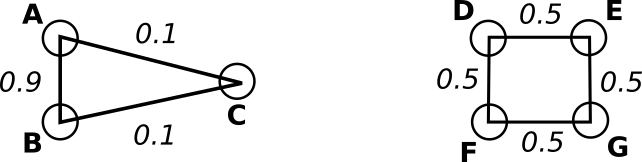
\includegraphics[width=0.5\textwidth]{ExampleGraph.png}
    \caption{Toy example}
\end{figure}
\begin{equation*}
L = \begin{bmatrix}
1  & -0.9 & -0.1 & 0 & 0 & 0 & 0 \\
-0.9 & 1  & -0.1 & 0 & 0 & 0 & 0 \\
-0.1 & -0.1 & 0.2  & 0 & 0 & 0 & 0 \\
0    & 0    & 0    & 1 & -0.5 & -0.5 & 0 \\
0    & 0    & 0    & -0.5 & 1 & 0 & -0.5 \\
0    & 0    & 0    & -0.5 & 0 & 1 & -0.5 \\
0    & 0    & 0    & 0 & -0.5 & -0.5 & 1 \\ 
\end{bmatrix}
\end{equation}
\end{frame}
\begin{frame}
\frametitle{Spectral Graph Partitioning}
\label{sec-2-5}

\vspace*{-0.0cm}\begin{figure}
      \subfigure[$\lambda_1 = 0$]{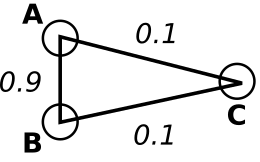
\includegraphics[width=0.15\textwidth]{ExampleGraphEvec1.png}}
      \subfigure[$\lambda_2 = 0$]{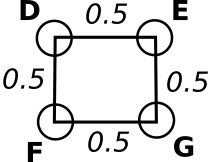
\includegraphics[width=0.15\textwidth]{ExampleGraphEvec2.png}}
\end{figure}
\vspace*{-0.0cm}\begin{figure}
      \subfigure[$\lambda_3$]{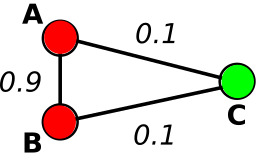
\includegraphics[width=0.15\textwidth]{ExampleGraphEvec3.png}}
      \subfigure[$\lambda_4$]{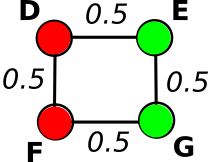
\includegraphics[width=0.15\textwidth]{ExampleGraphEvec4.png}}
      \subfigure[$\lambda_5$]{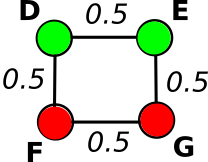
\includegraphics[width=0.15\textwidth]{ExampleGraphEvec5.png}}
\end{figure}
\begin{itemize}
\item Two zero eigenvalues, corresponding to two clusters
\item Eigenvalues close to zero give good partitions within clusters
\end{itemize}
\end{frame}
\section{Application to Icing}
\label{sec-3}
\begin{frame}
\frametitle{Dataset}
\label{sec-3-1}

\vspace*{-0.0cm}\begin{figure}
      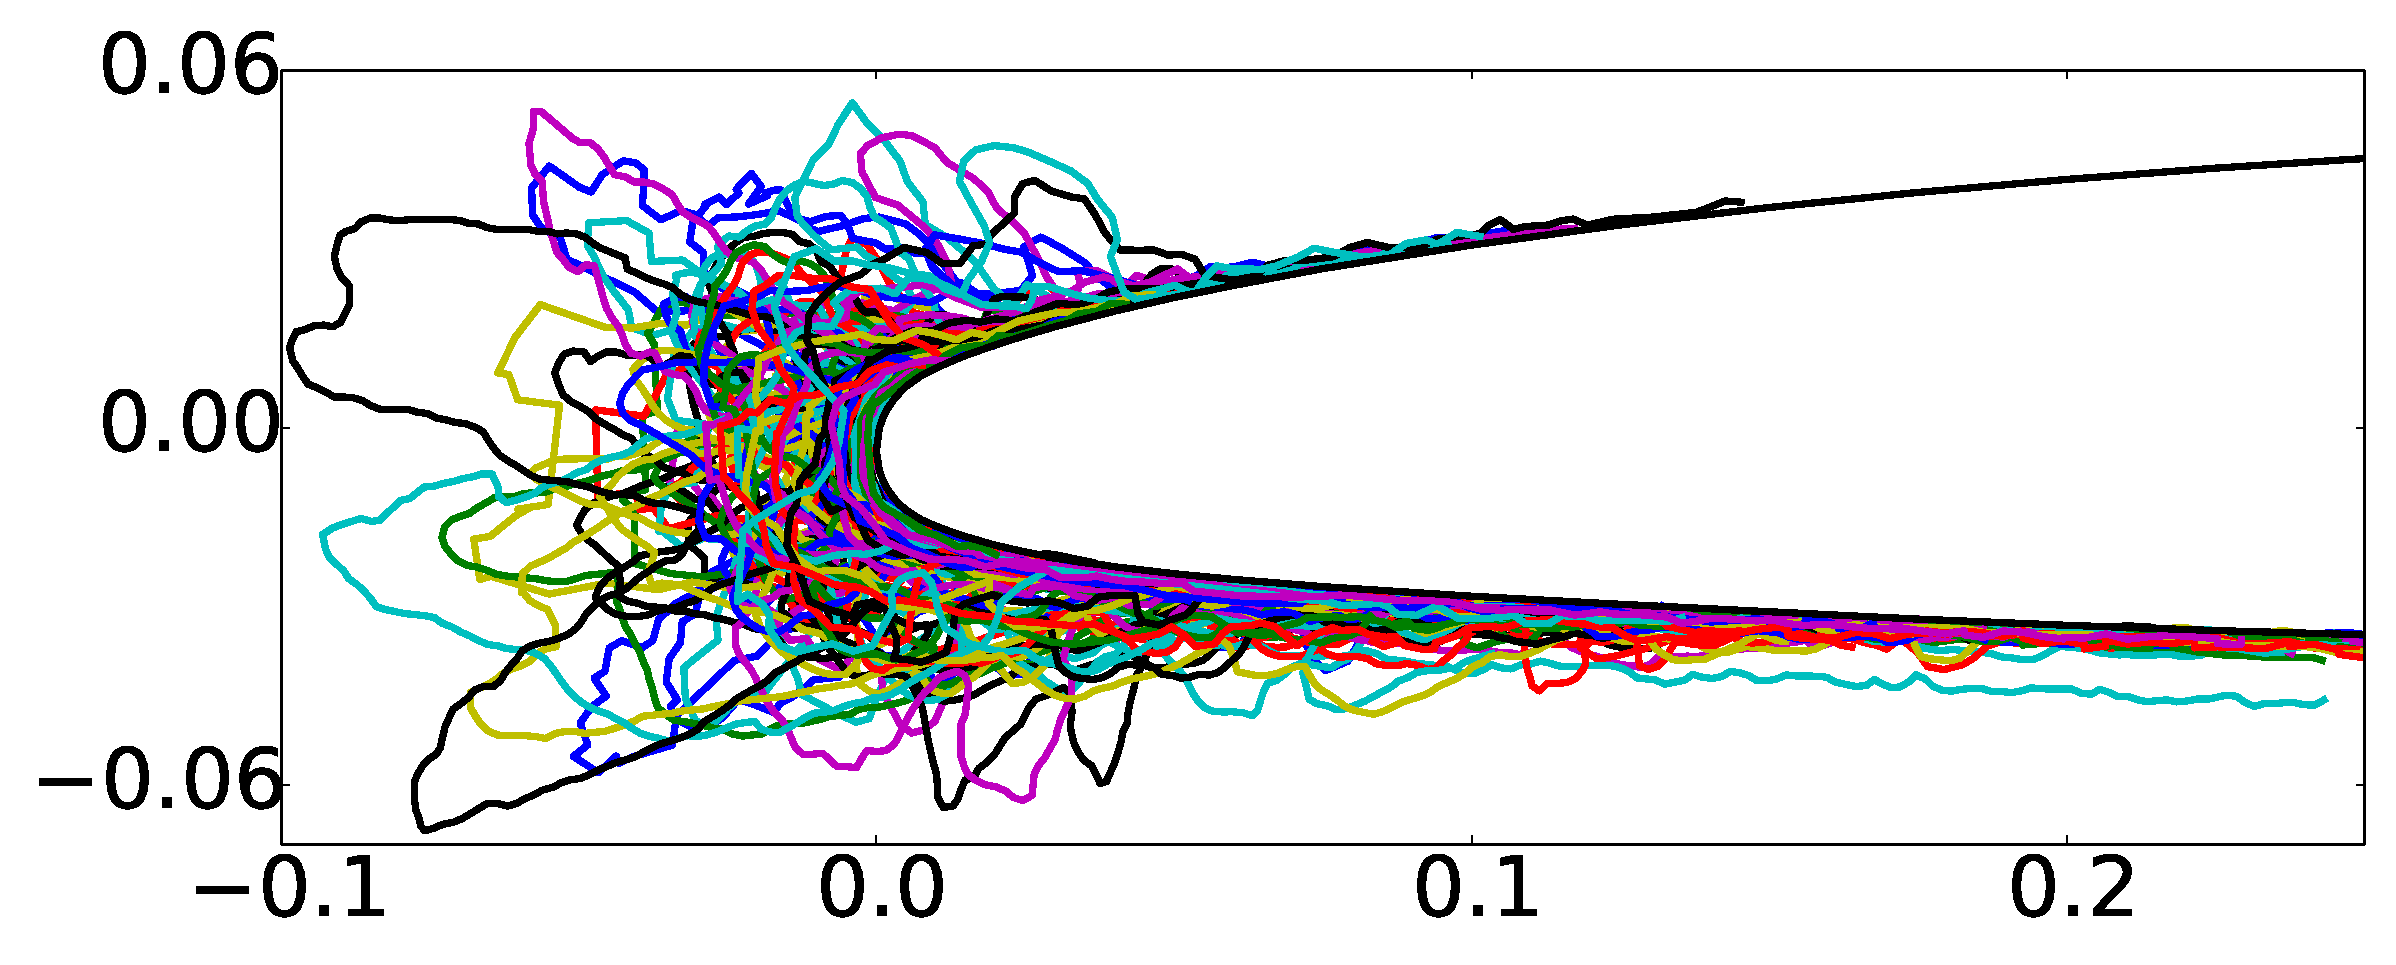
\includegraphics[width=0.5\textwidth]{GlobalDataSet}
      \caption{Wind tunnel experimental ice shapes}
\end{figure}
\begin{itemize}
\item Dataset consists of 145 experimental ice shapes
\item Obtained in icing wind tunnel at NASA Glenn\footnotemark[1]
\item Representative of a wide variety of icing conditions (temperature,
  LWC, accretion time, etc.)
\end{itemize}
\end{frame}
\begin{frame}
\frametitle{Distance/Similarity Metric}
\label{sec-3-2}

\vspace*{-0.0cm}\begin{figure}
      \subfigure[XOR Illustration]{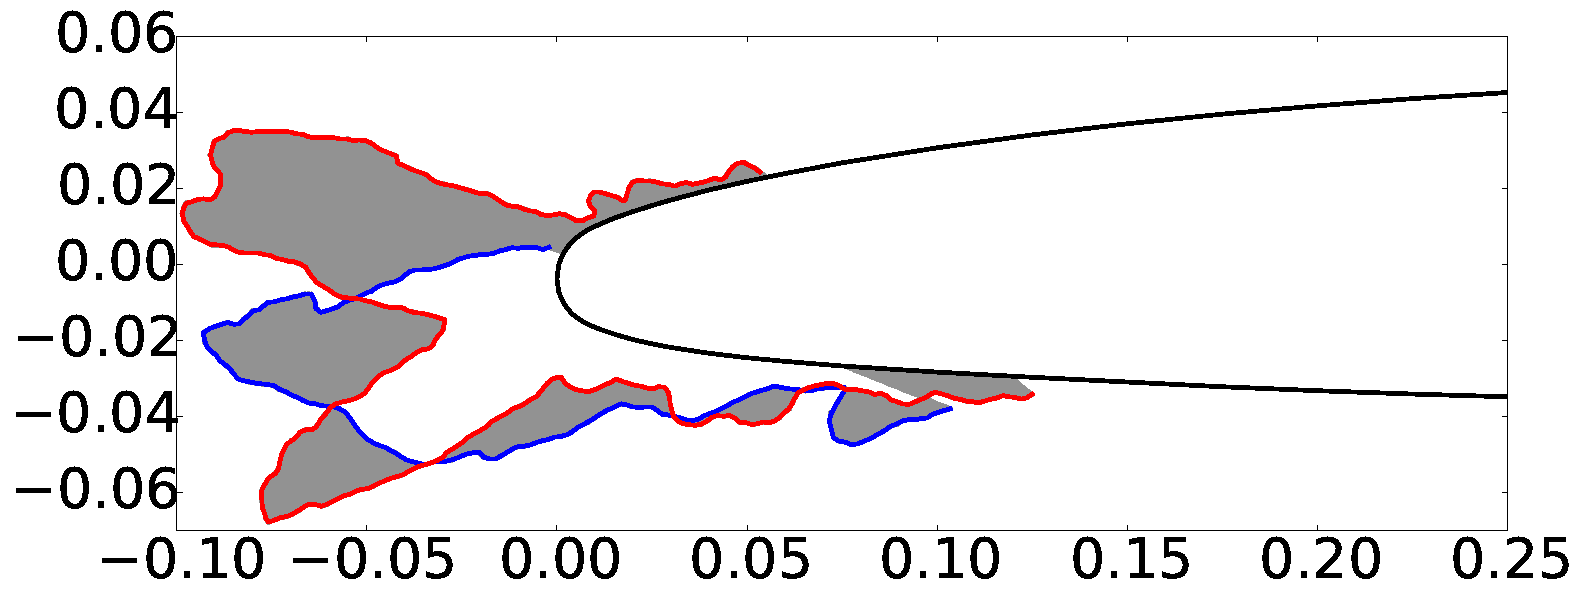
\includegraphics[width=0.4\textwidth]{XORexample.png}}
      \subfigure[Dataset Distances]{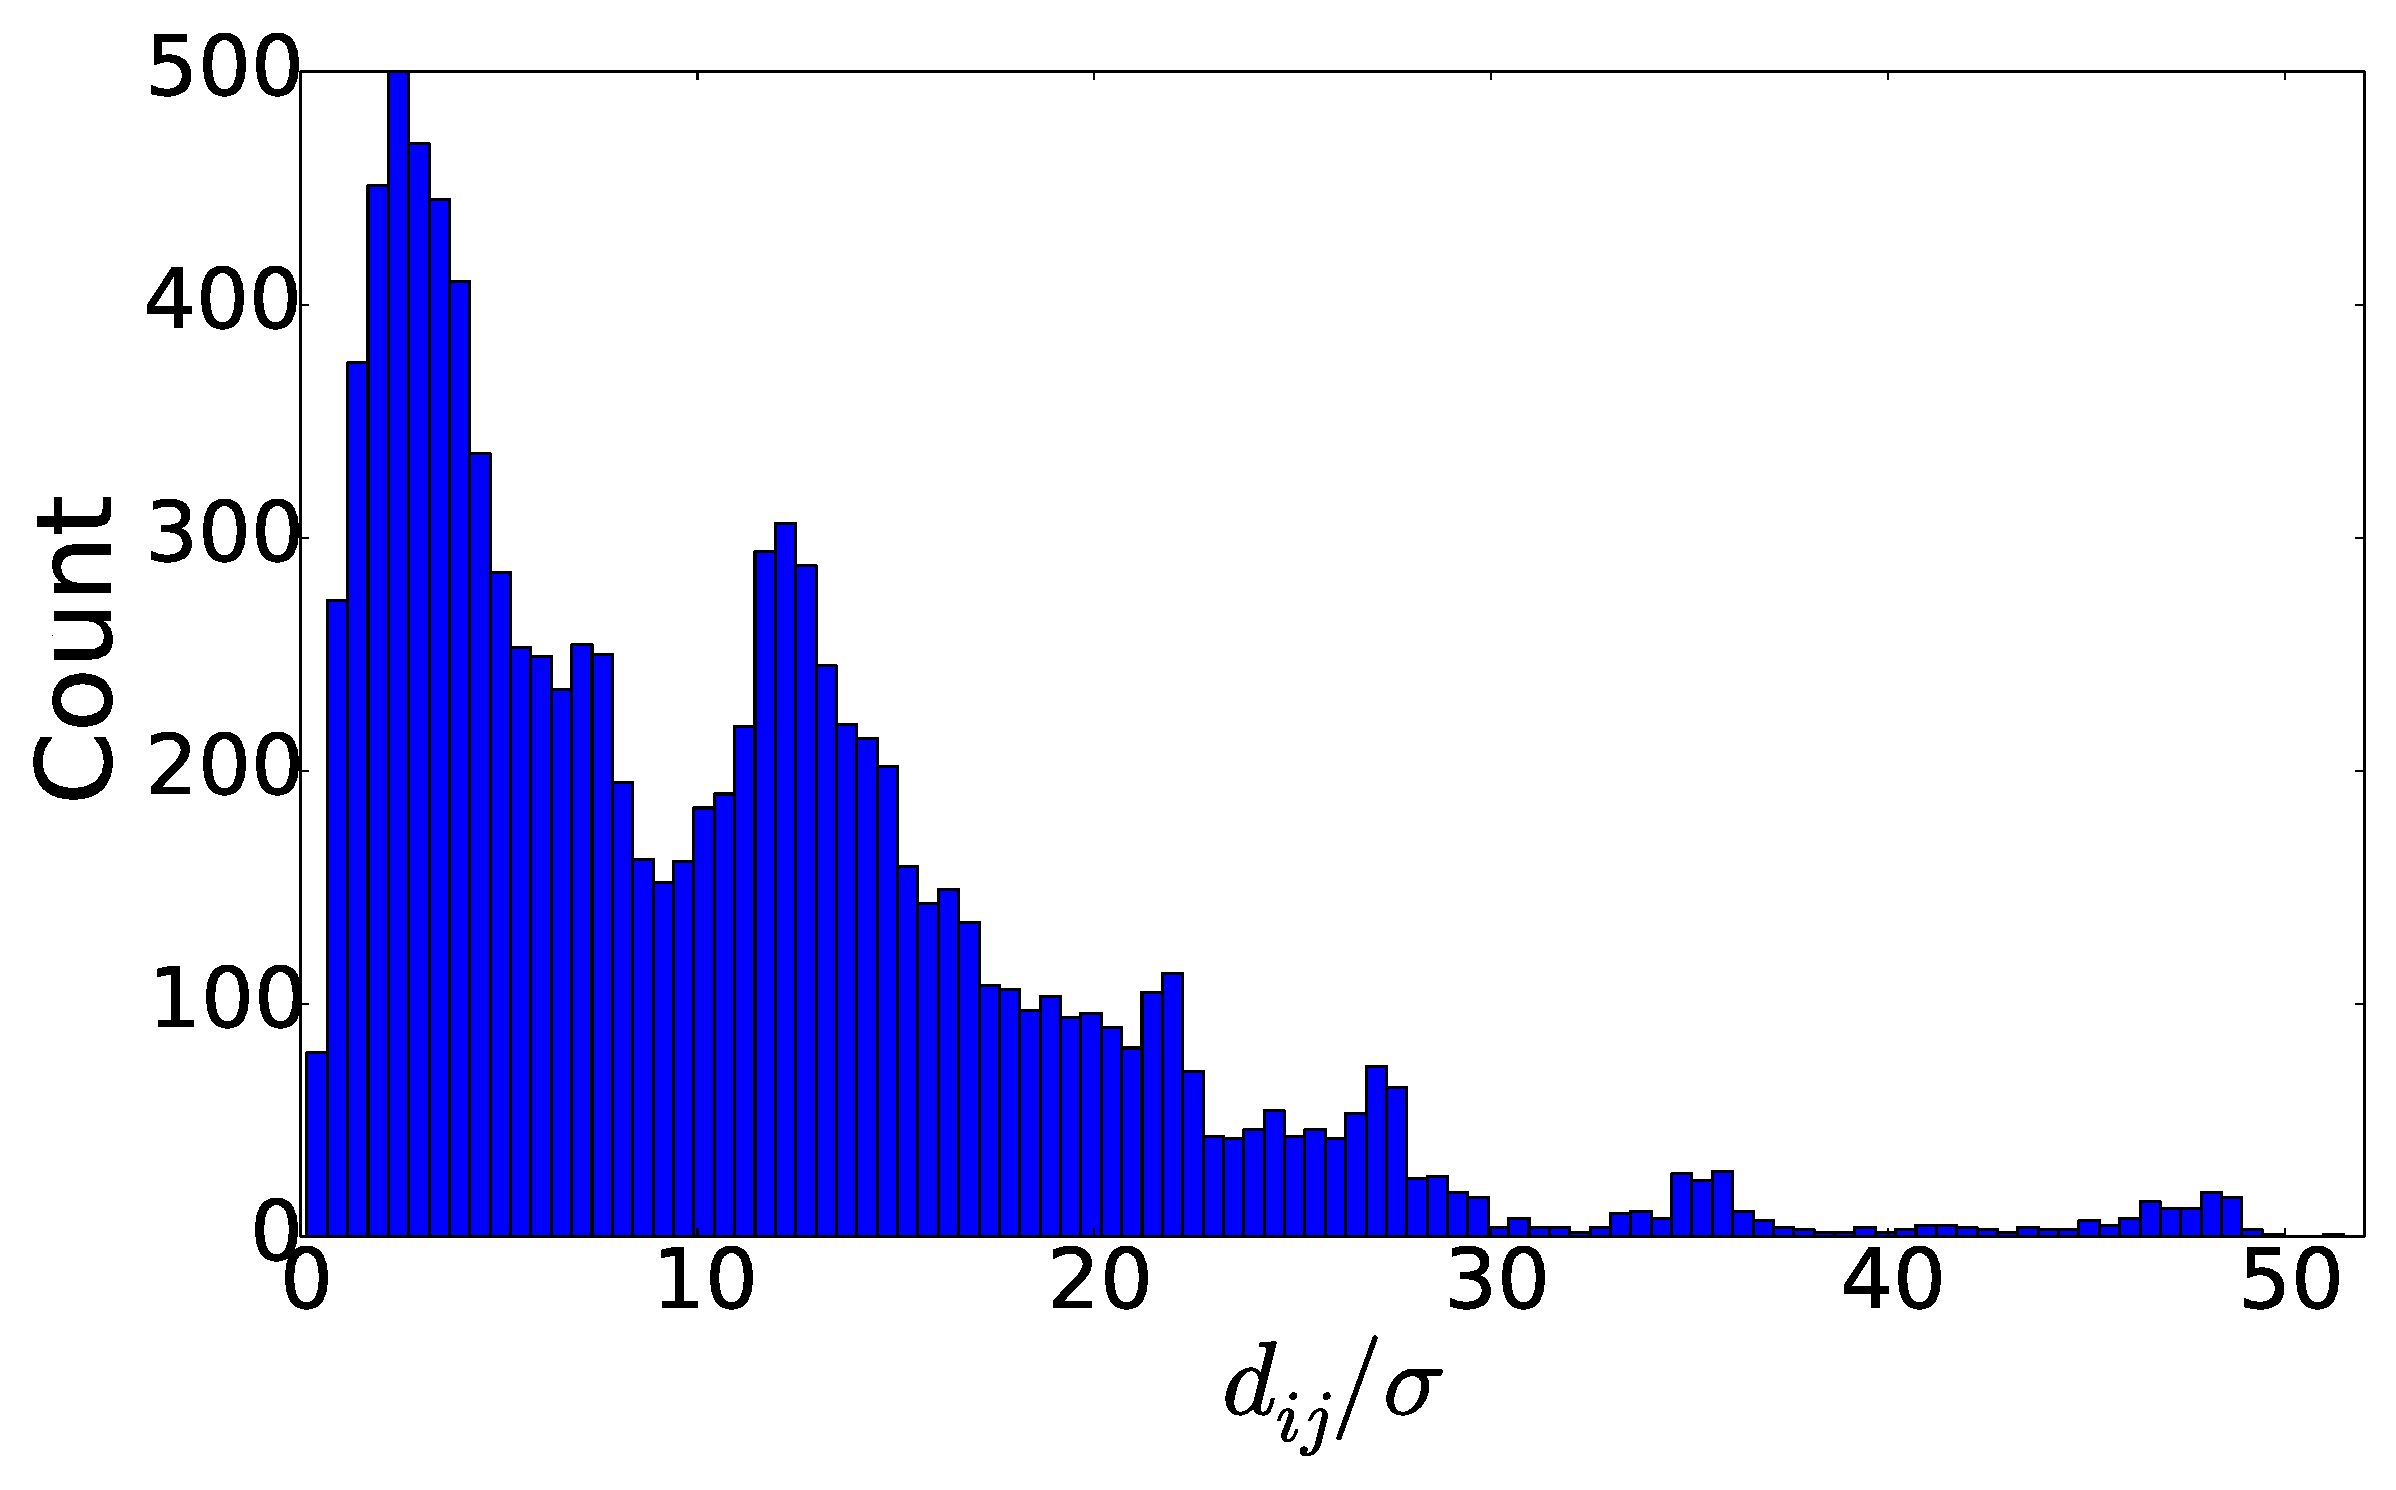
\includegraphics[width=0.4\textwidth]{XORdistances}}
\end{figure}
\begin{itemize}
\item Overlay dataset with a 2D Cartesian grid
\item Assign value of 1 to gridpoint if it is on the ice, 0 otherwise
\item Pick $\sigma$ based on observed peaks in data distances
\item Truncate $w_{ij}$ after $d_{ij} > 3\sigma$
\end{itemize}
\begin{equation*}
\begin{aligned}
d_{ij} &= \text{exp} \left(-\frac{1}{2} \frac{d_{ij}^2}{\sigma^2} \right) \\
w_{ij} &= \sum_k^{N_G} \left [ \text{XOR}(x_i,x_j) \right ]_k
\end{aligned}
\end{equation}
 
\end{frame}
\begin{frame}
\frametitle{Graph Laplacian}
\label{sec-3-3}

\vspace*{-0.0cm}\begin{figure}
      \subfigure[Graph Laplacian]{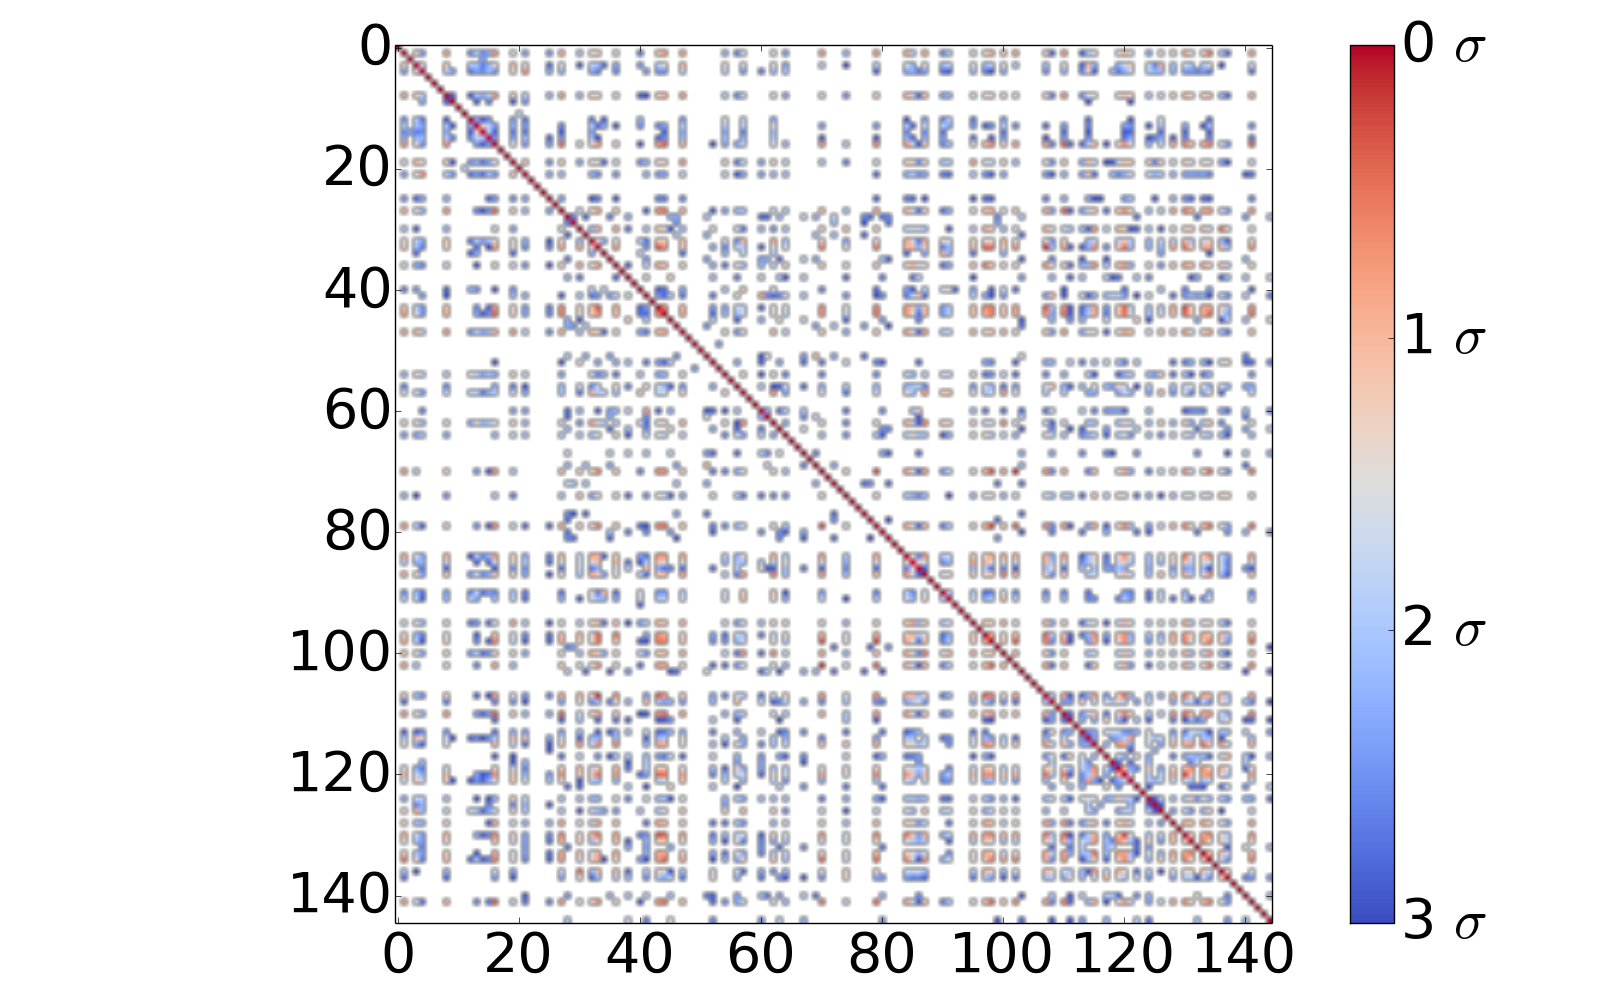
\includegraphics[width=0.4\textwidth]{DistanceMatrixUnordered.png}}
      \subfigure[Eigenvalue Magnitudes]{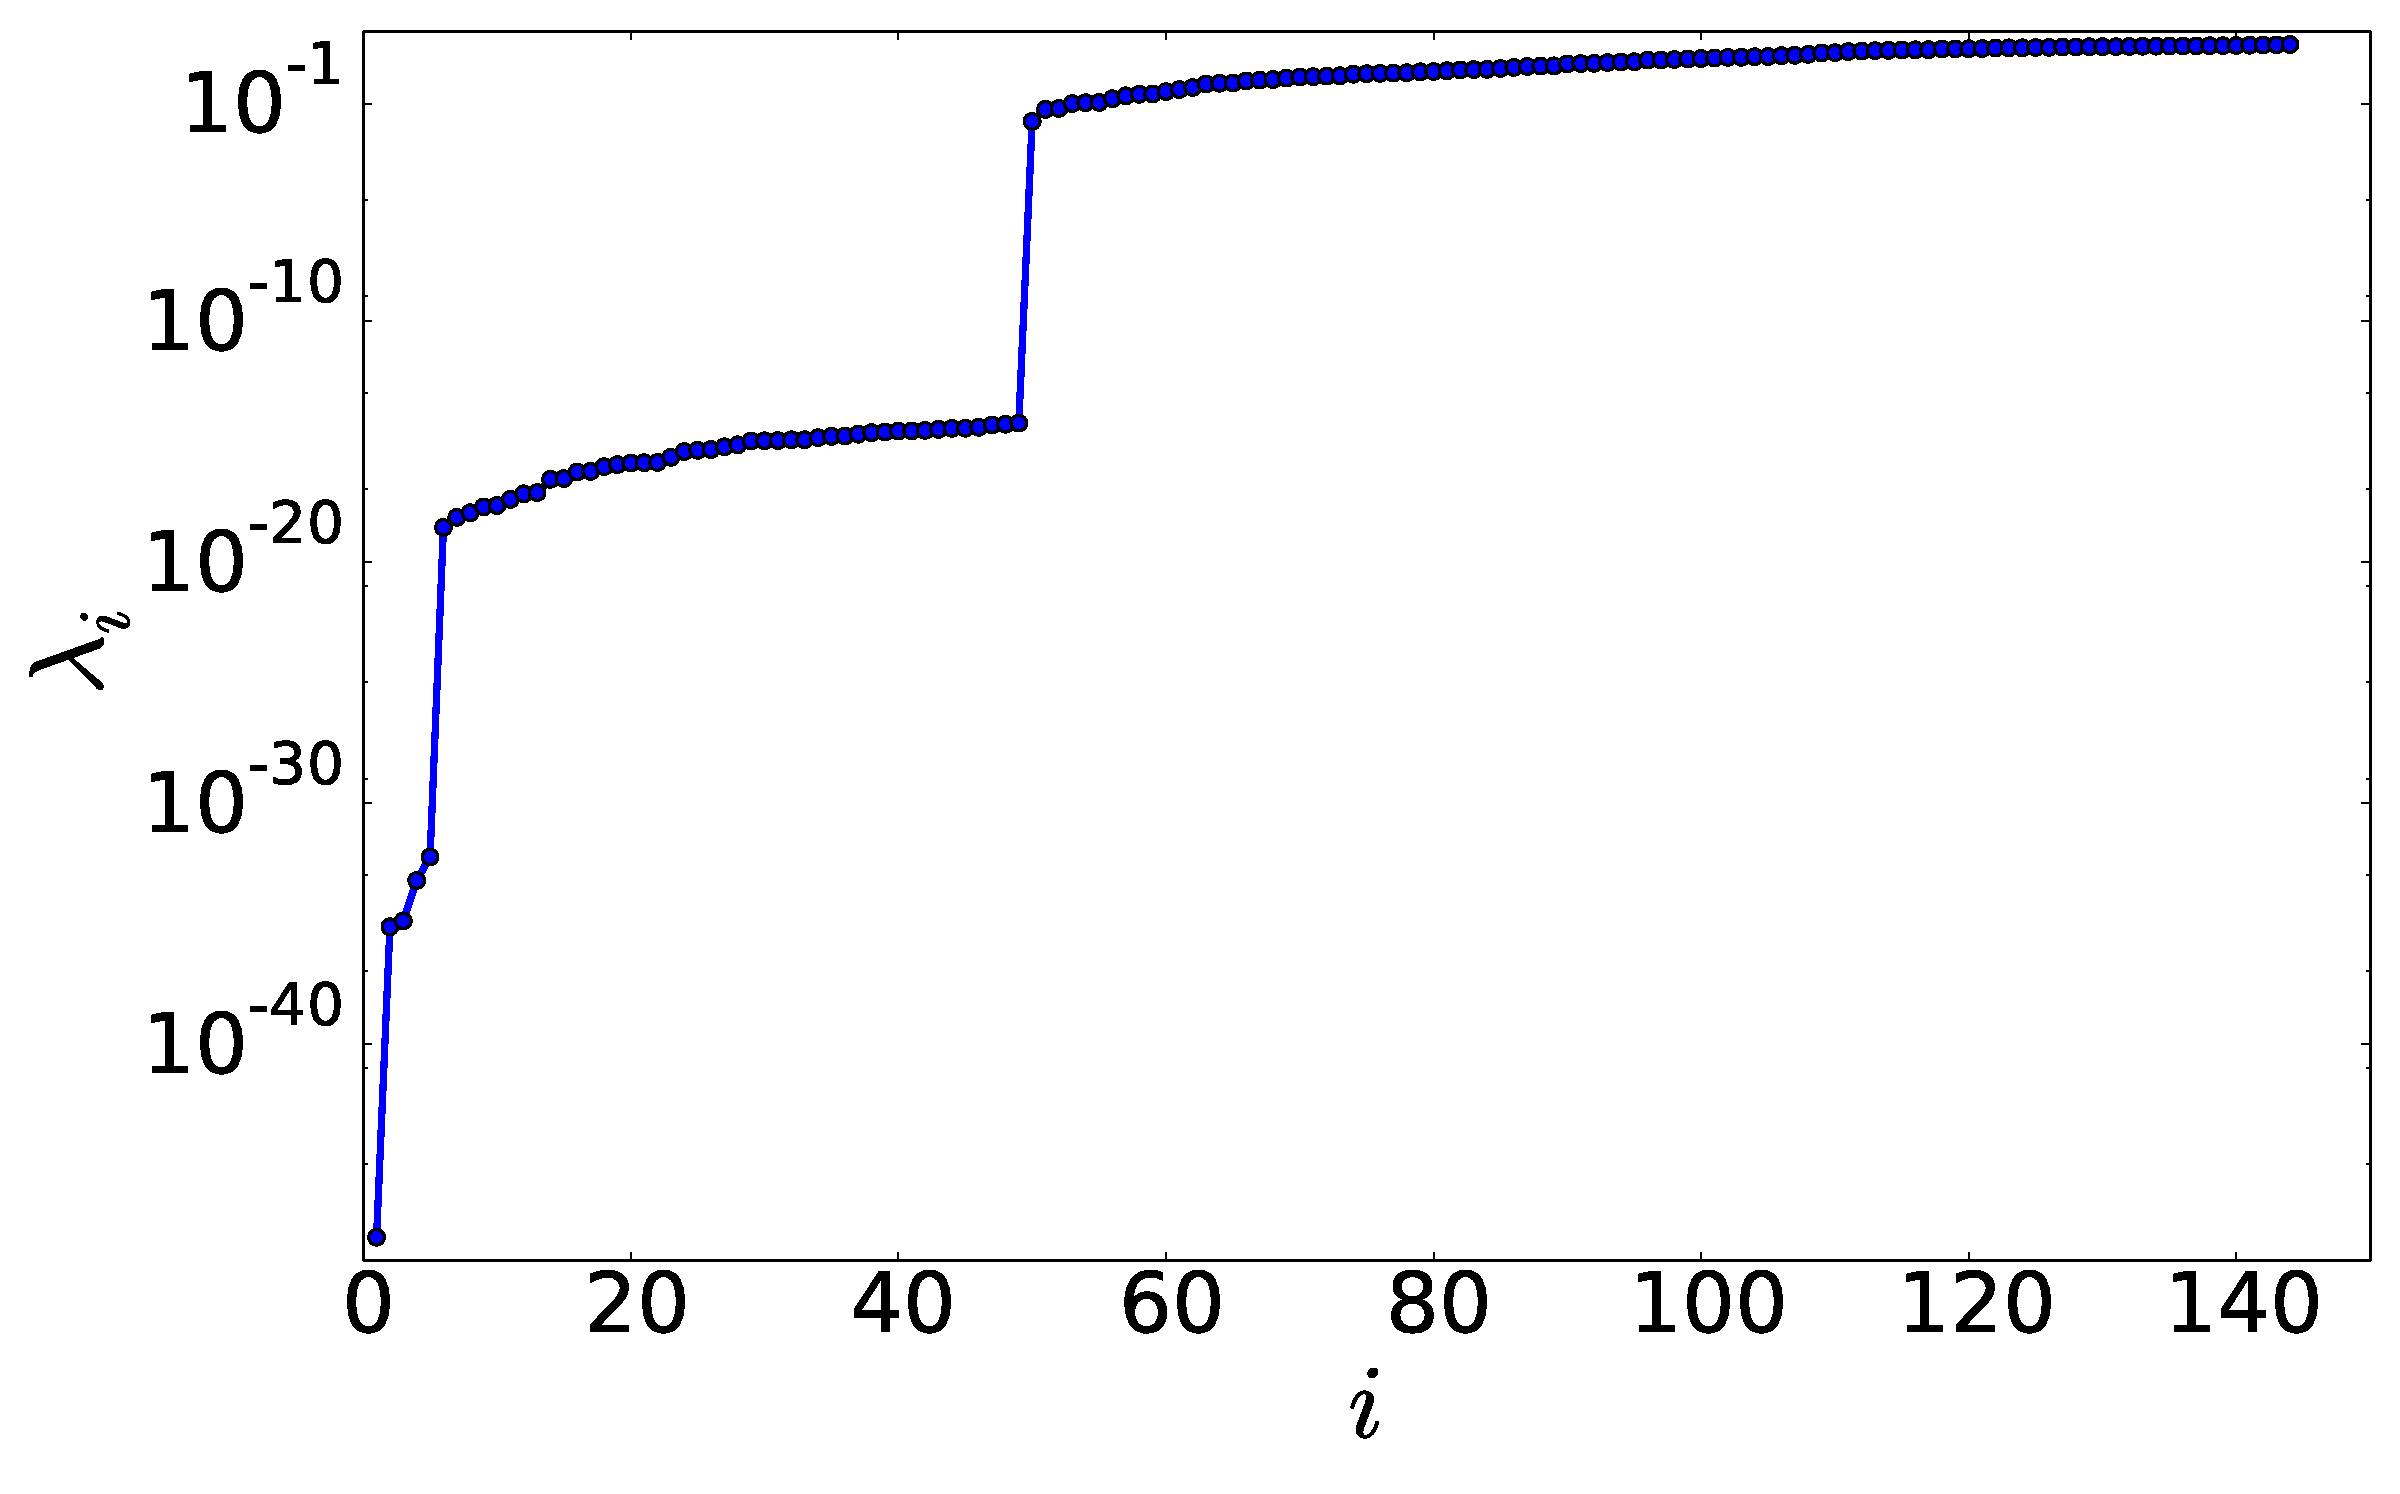
\includegraphics[width=0.4\textwidth]{LaplacianEvals}}
\end{figure}
\begin{itemize}
\item Many zero eigenvalues because many of the dataset elements are
  completely unconnected from each other
\end{itemize}
\end{frame}
\begin{frame}
\frametitle{Clusters}
\label{sec-3-4}

\vspace{-1.0cm}
\begin{columns}[c]
  \column{0.3\textwidth}
    \centering
    \vspace*{-0.0cm}\begin{figure}
      \subfigure[]{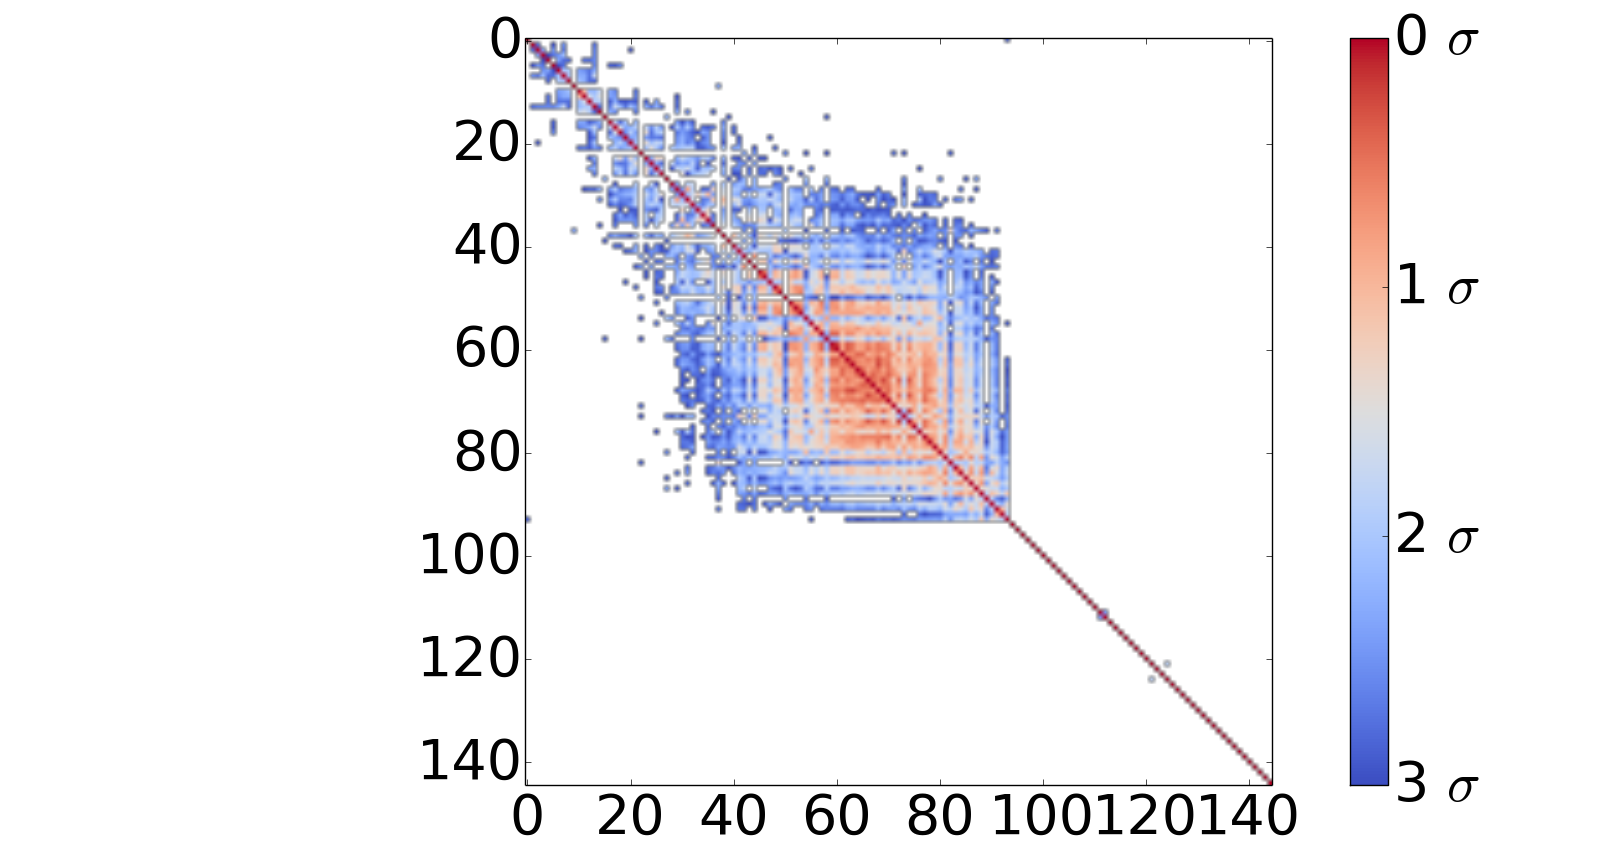
\includegraphics[width=0.95\textwidth]{DistanceMatrixOrdered.png}}
      \subfigure[]{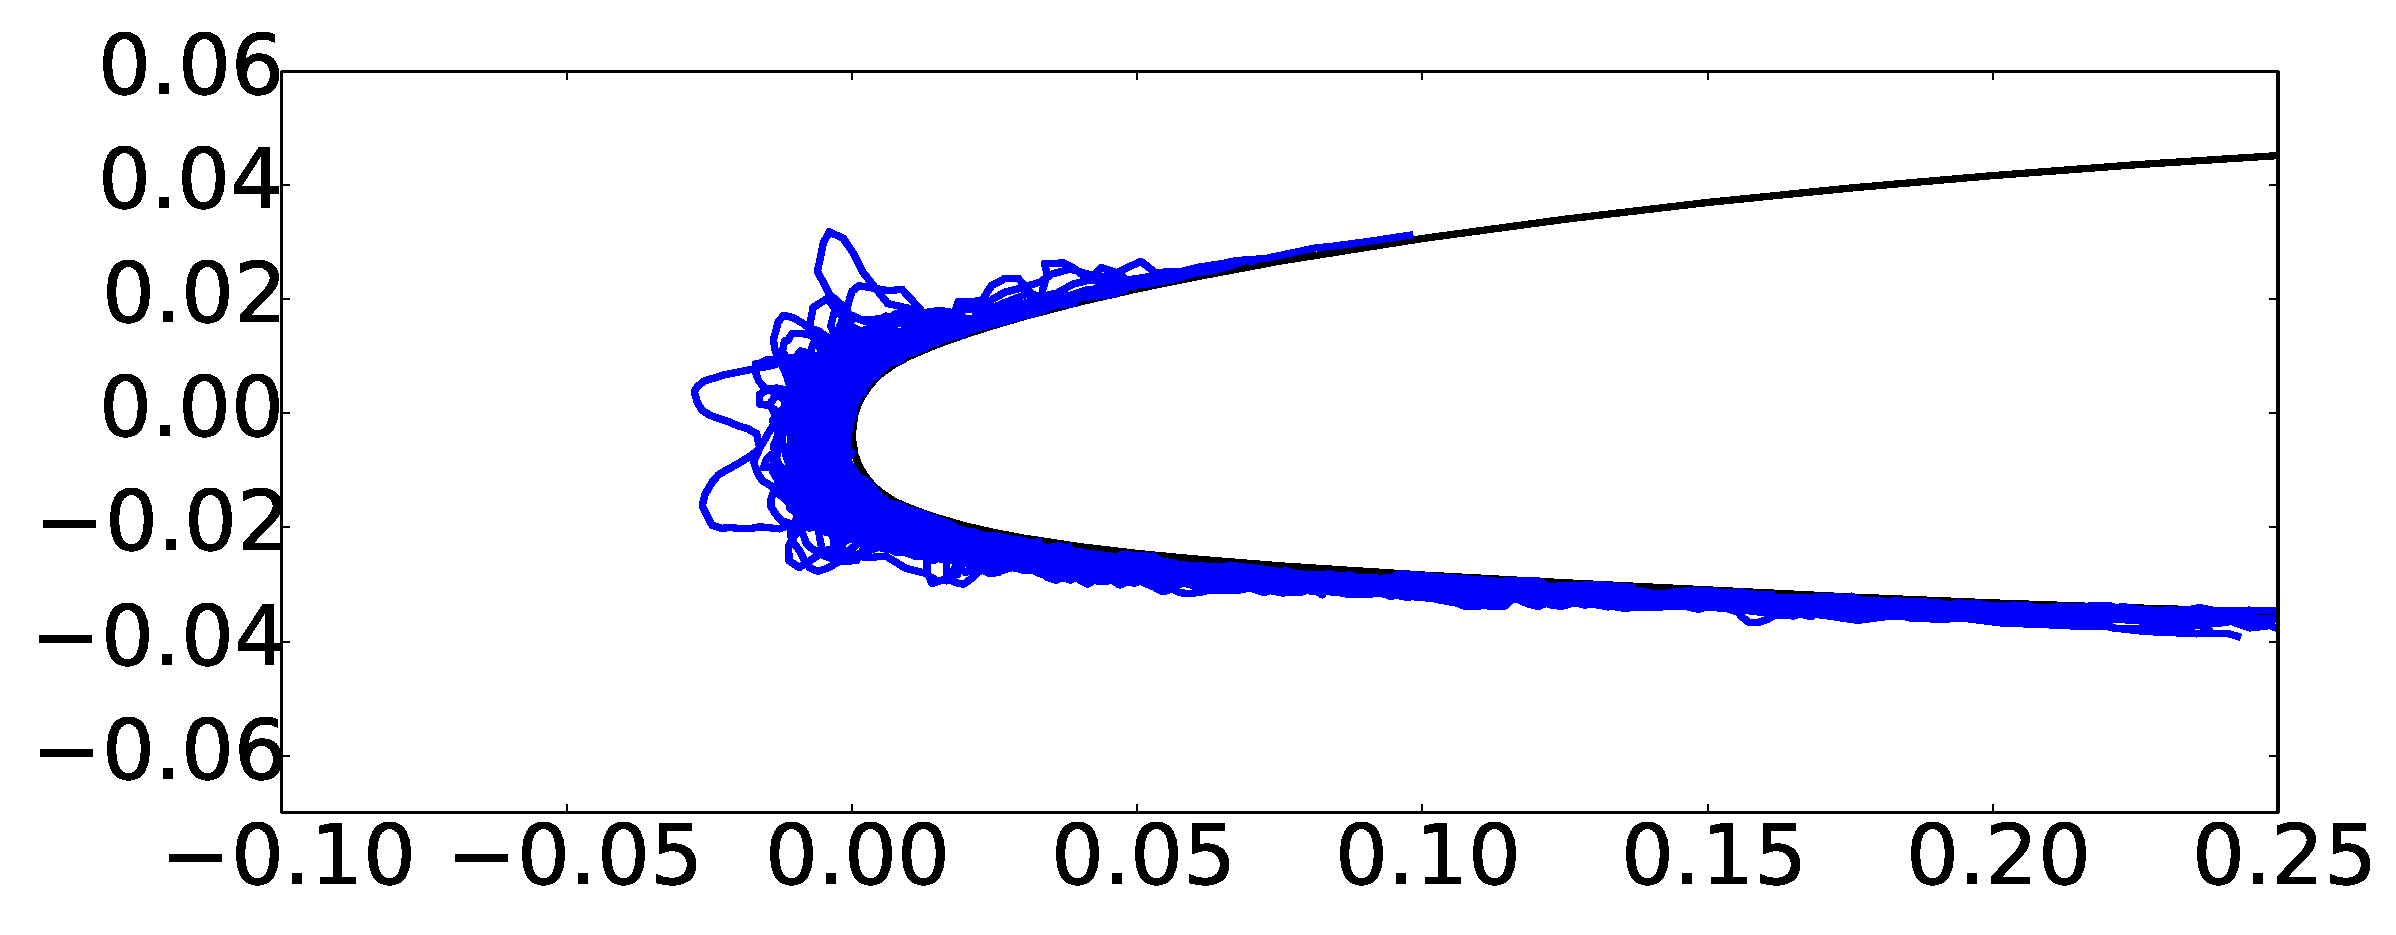
\includegraphics[width=0.95\textwidth]{LaplacianUnconnectedCluster}}
      \caption{$\lambda = 0$}
    \end{figure}    
  \column{0.3\textwidth}
    \centering
    \vspace*{-0.0cm}\begin{figure}
      \subfigure[]{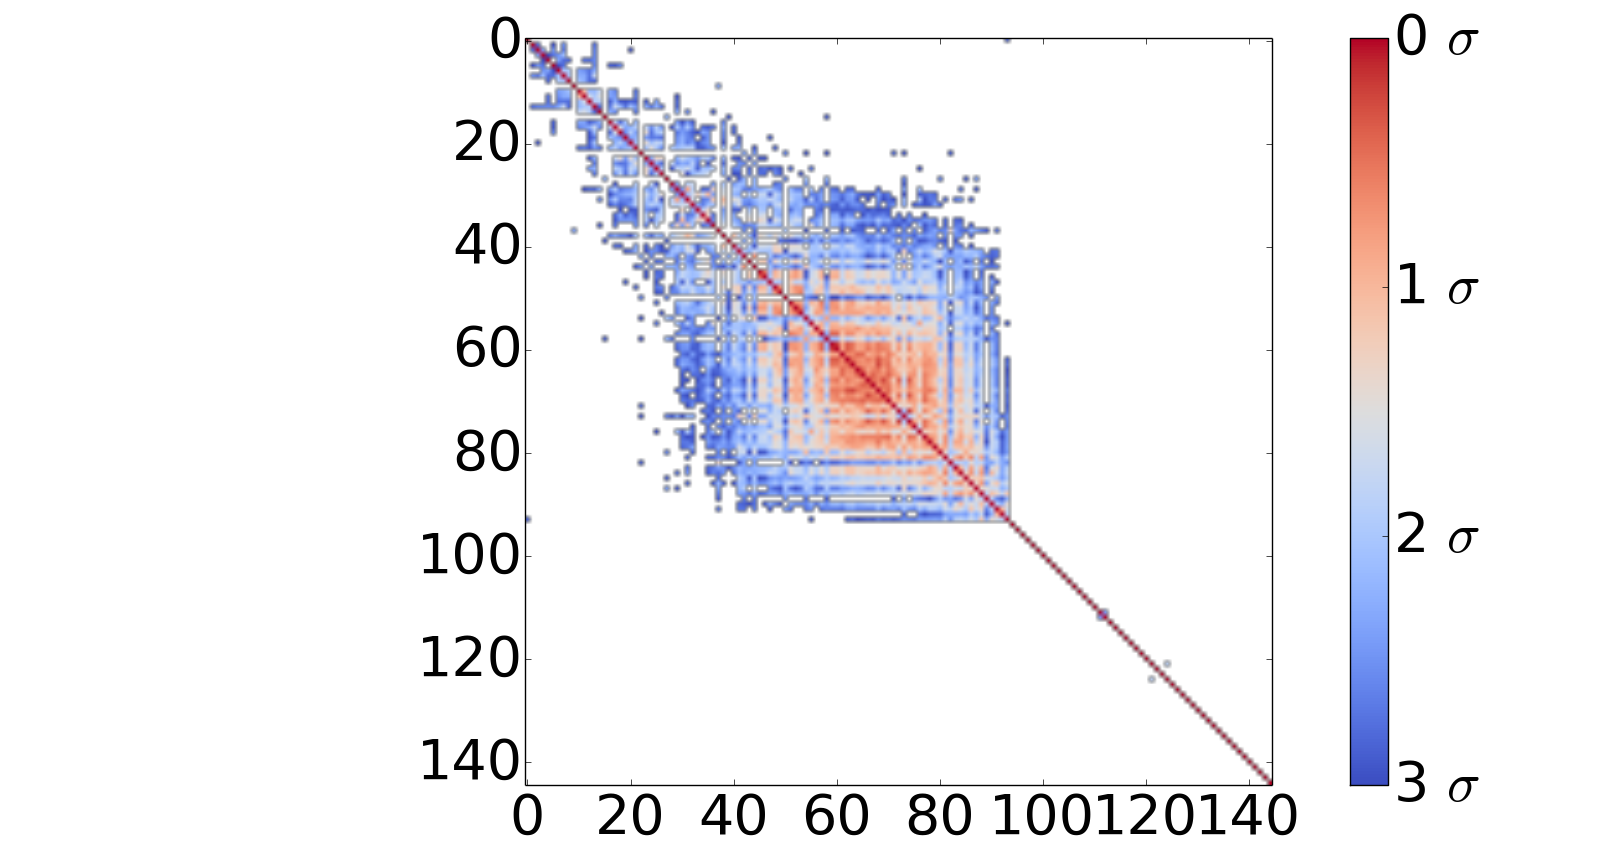
\includegraphics[width=0.95\textwidth]{DistanceMatrixOrdered.png}}
      \subfigure[]{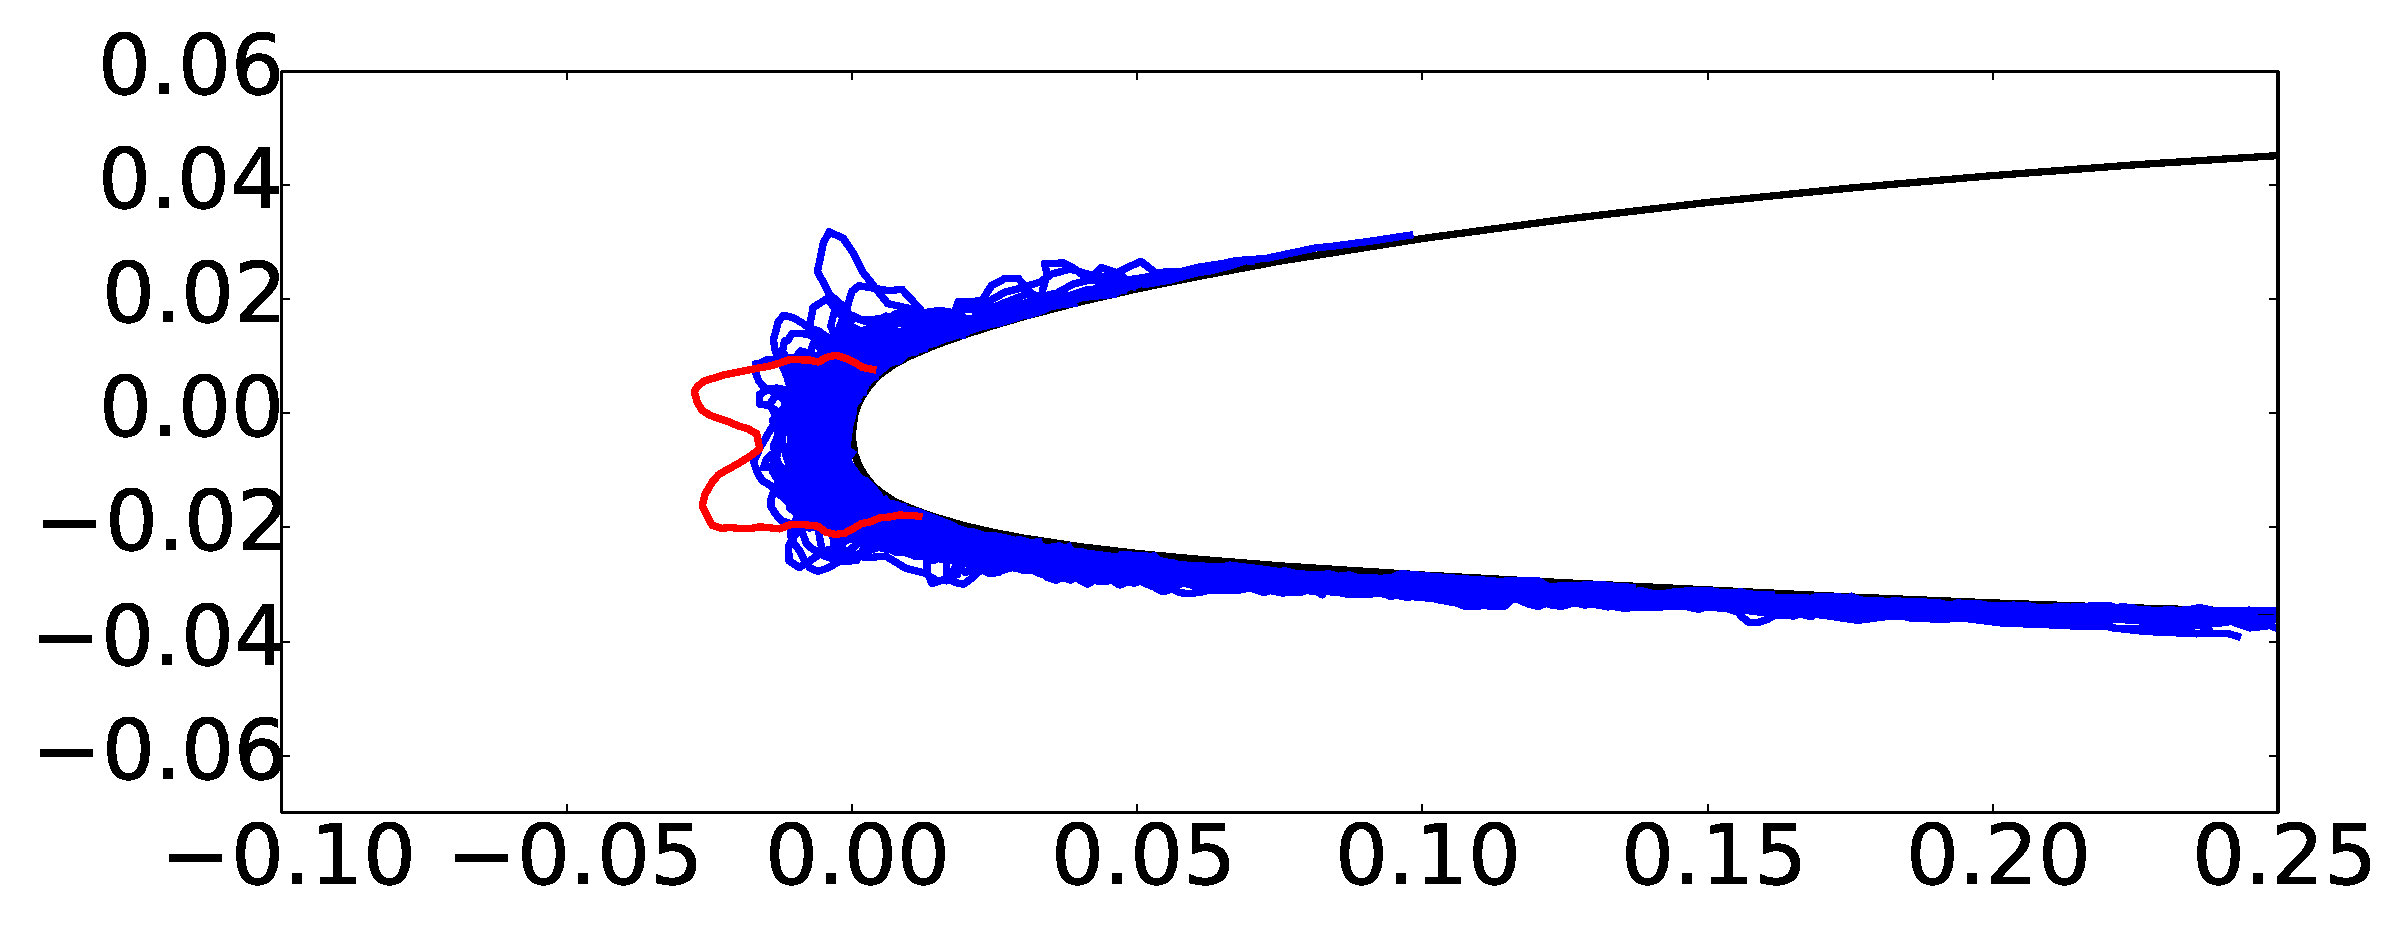
\includegraphics[width=0.95\textwidth]{FiedlerVectorGrouping}}
      \caption{Fiedler Vector}
    \end{figure}
  \column{0.3\textwidth}
    \centering
    \vspace*{-0.0cm}\begin{figure}
      \subfigure[]{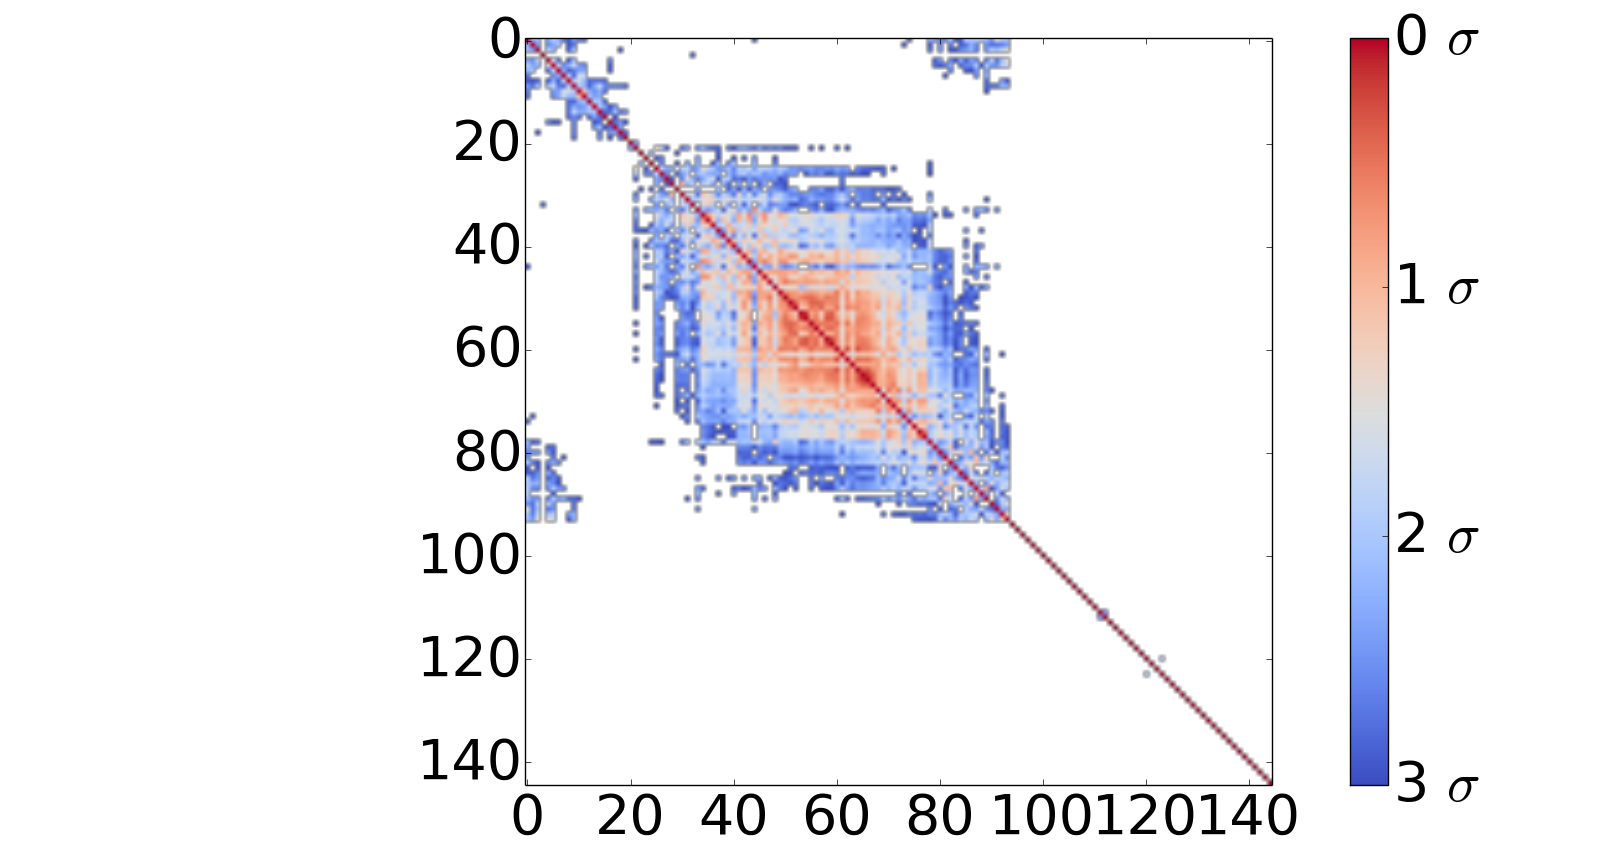
\includegraphics[width=0.95\textwidth]{DistanceMatrixOrdered2.png}}
      \subfigure[]{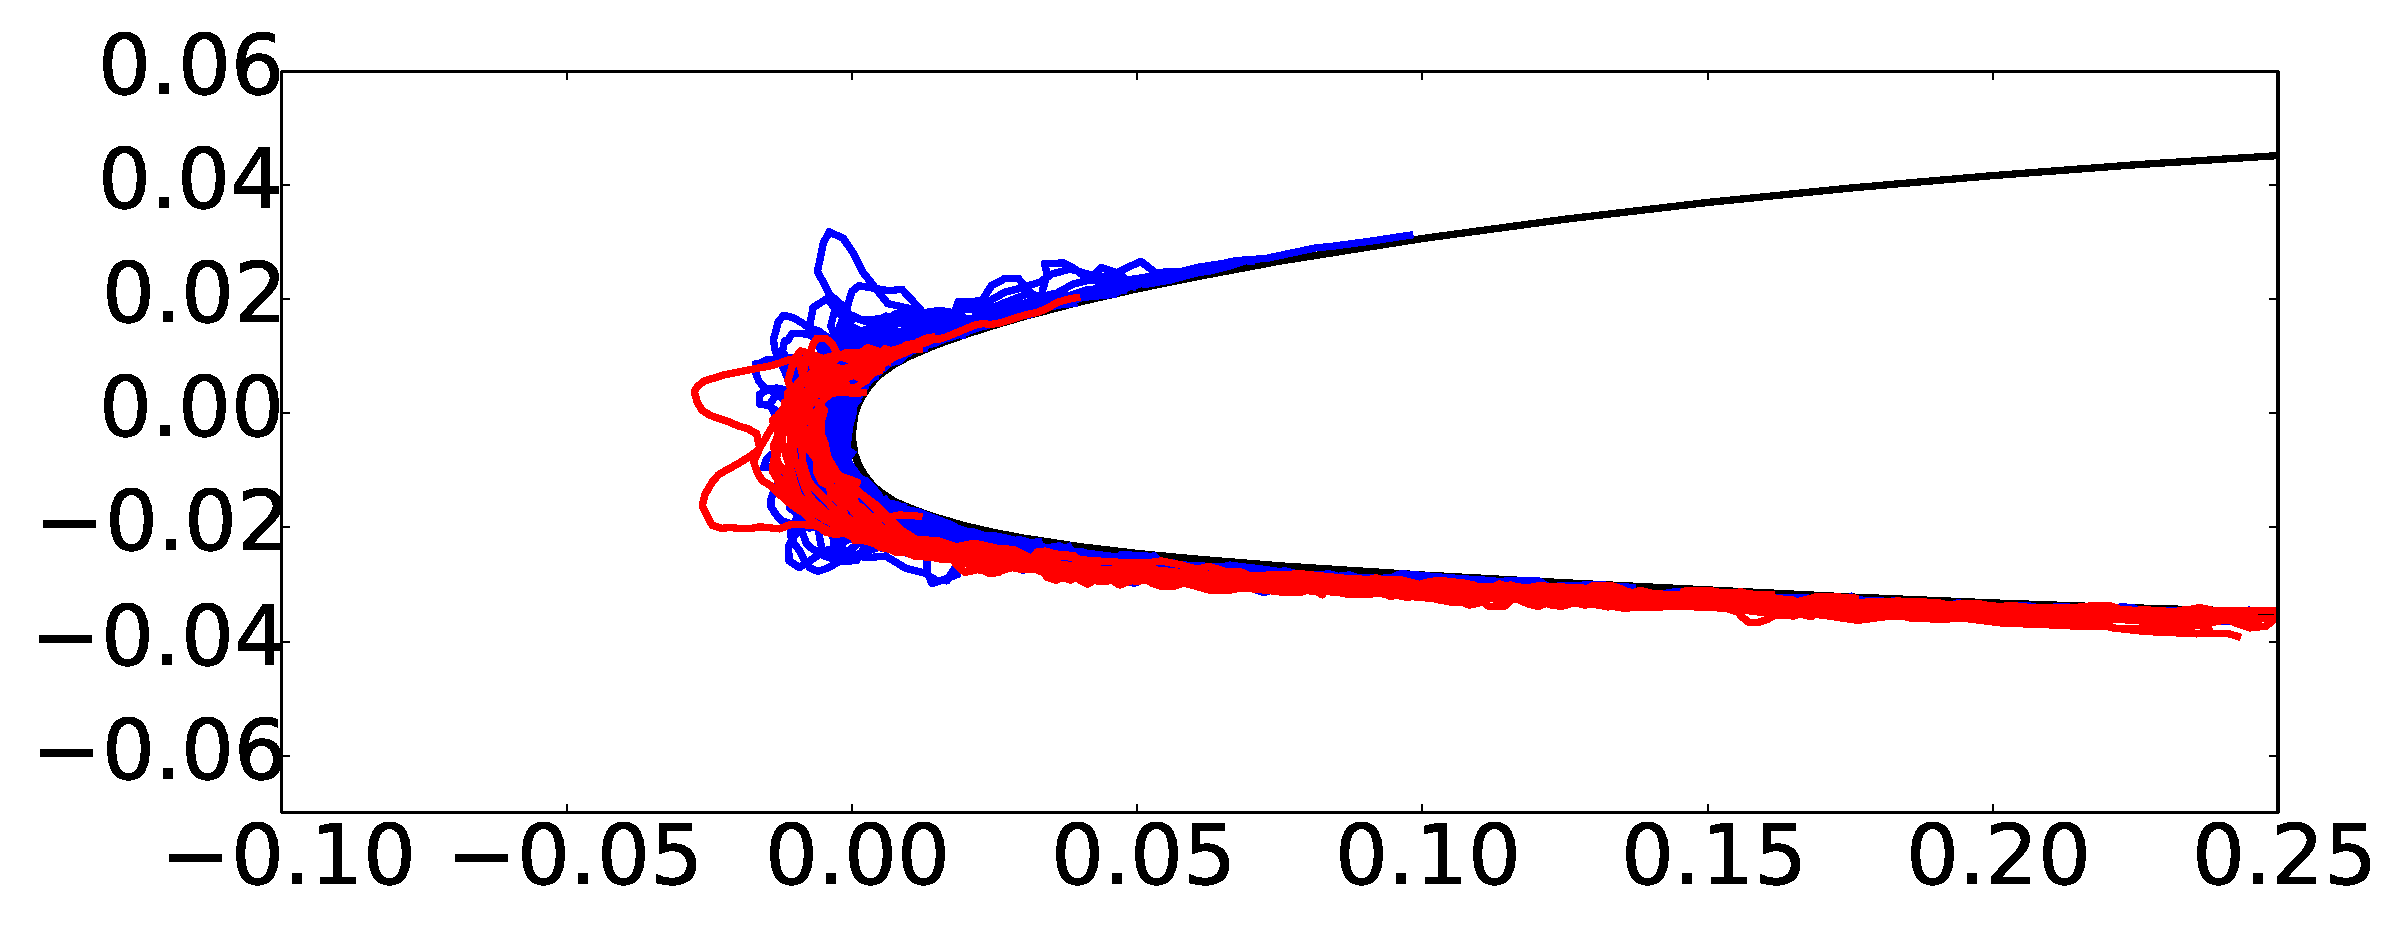
\includegraphics[width=0.95\textwidth]{Fiedler2VectorGrouping}}
      \caption{Next eigenvector}
    \end{figure}
\end{columns}
\begin{itemize}
\item Unconnected cluster represents smaller and less ``extreme'' shapes
\item Fiedler vector partitions off single most dissimilar member
\item Next smallest eigenvector separates horn and rime accretion
\end{itemize}
\end{frame}
\begin{frame}
\frametitle{POD Coordinates}
\label{sec-3-5}

\vspace*{-0.0cm}\begin{figure}
    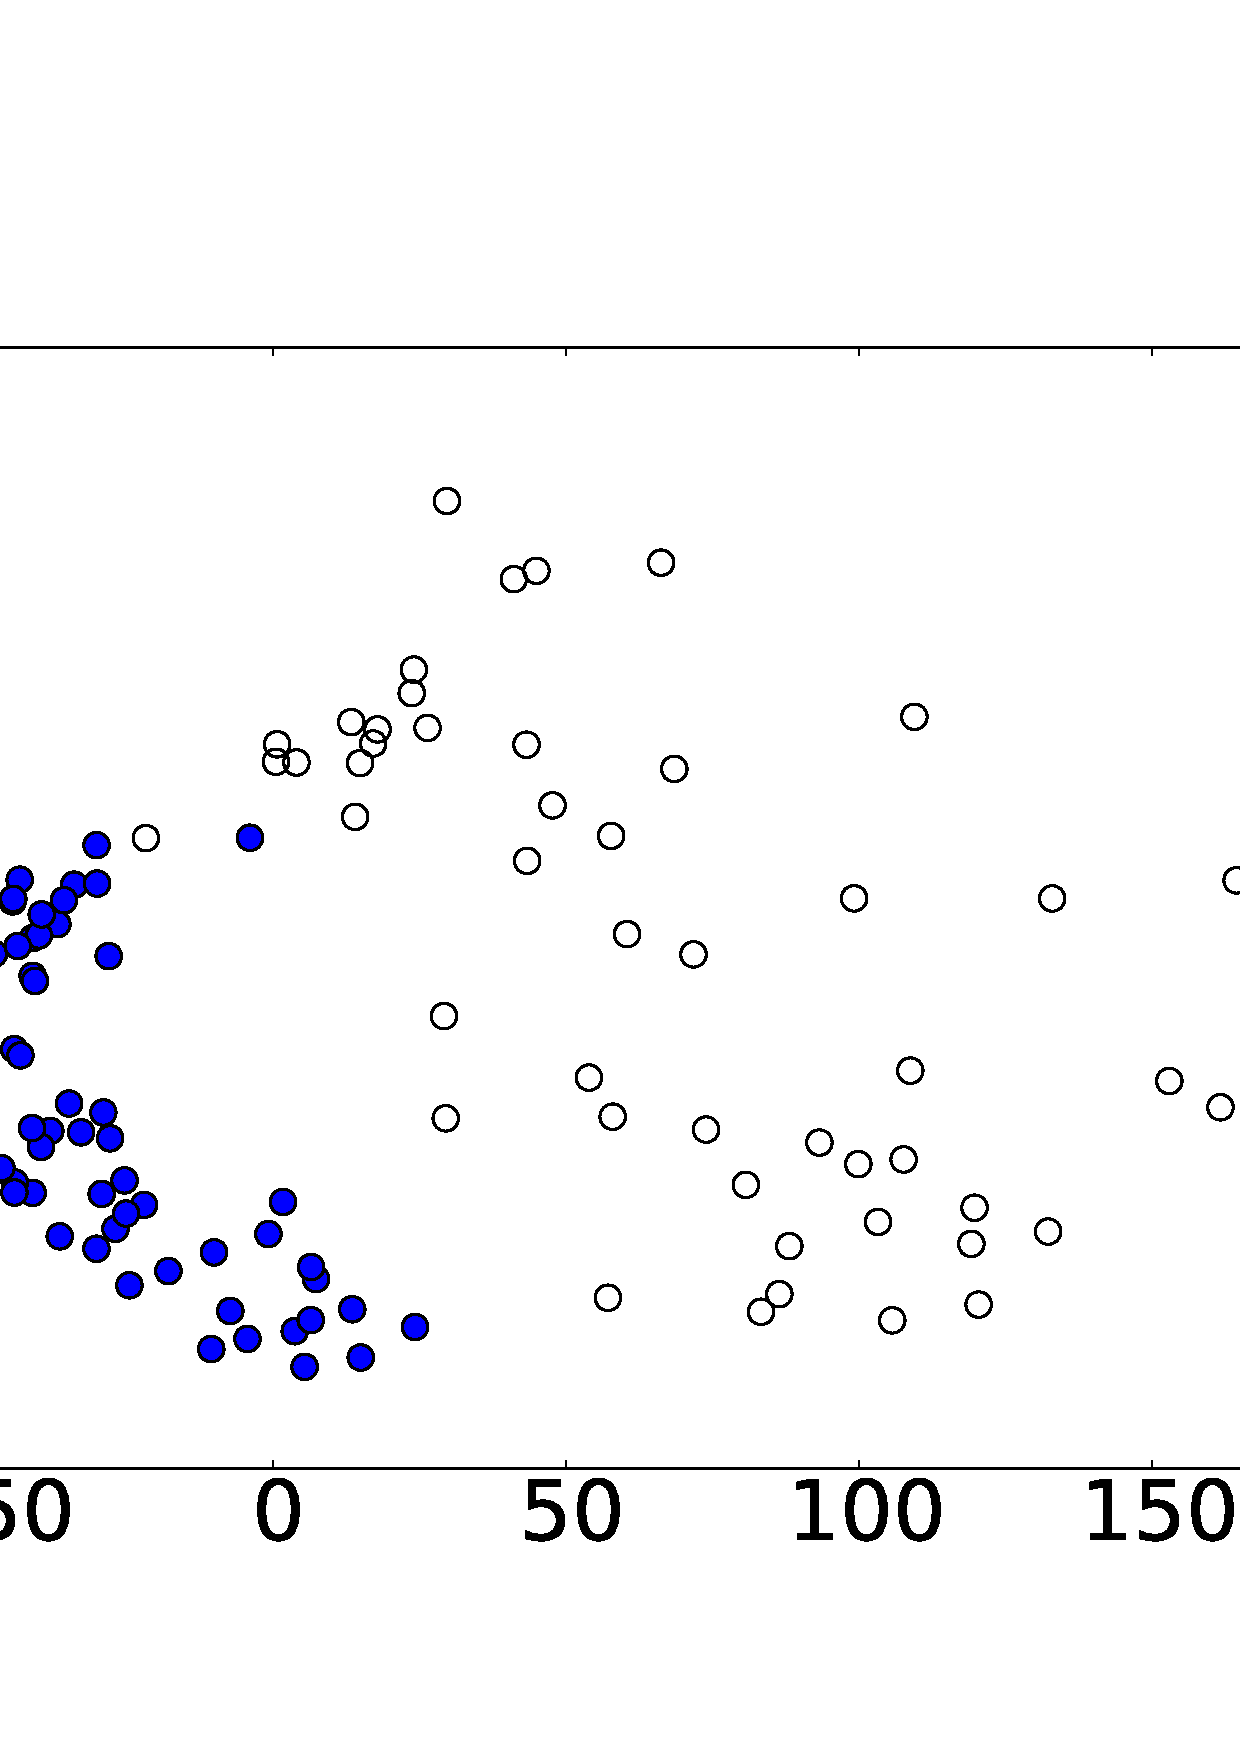
\includegraphics[width=0.4\textwidth]{ClusterPODcoords.png}
    \caption{POD coordinates of shapes ({\it red}) and cluster ({\it blue})}
\end{figure}
\end{frame}
\section{Uncertainty Quantification}
\label{sec-4}
\begin{frame}
\frametitle{POD Model}
\label{sec-4-1}
\end{frame}
\begin{frame}
\frametitle{POD Model}
\label{sec-4-2}
\end{frame}
\begin{frame}
\frametitle{Parameter Space}
\label{sec-4-3}
\end{frame}
\begin{frame}
\frametitle{Output Statistics}
\label{sec-4-4}
\end{frame}
\begin{frame}
\frametitle{Global Extrema}
\label{sec-4-5}
\end{frame}
\begin{frame}
\frametitle{Local Sensitivity}
\label{sec-4-6}
\end{frame}

\end{document}
